% !TeX root = thesis.tex
%---------------------------------------------------------------------------
% Vorlage für Bachelorarbeiten, Masterarbeiten
% der AG Autonome Intelligente Systeme
% Basierend auf der Vorlage der AG PRIA an der Universität Münster
% (Autoren dort: Daniel Tenbrinck, Fabian Gigengack, Michael Schmeing, Lucas Franek, Andreas Nienkötter
% Dazu Dank an Phil Steinhorst und dessen Vorlage, von der Teile übernommen wurden
%---------------------------------------------------------------------------

\documentclass[%
  paper=A4,               % Papiergröße
  twoside=true,           % zweiseitiges Layout
  openright,              % Kapitel auf ungerader Seite beginnen
  11pt,                   % Schriftgröße
  bibliography=totoc,     % Literaturverzeichnis im Inhaltsverzeichnis
  %listof=totoc,           % Abb.-/Tab.-verzeichnis im Inhaltsverzeichnis
  titlepage=on,           % Titel auf eigener Seite
  DIV=12,                 % Satzspiegelberechnung
  BCOR=1.5cm,             % Bindungskorrektur
  parskip=half,            % Absatzabstand
  final
]{scrreprt}

% Basics
\usepackage[x11names]{xcolor}

\usepackage{natbib}

% Schriftarten setzen
\usepackage[T1]{fontenc}
%\usepackage[utf8]{inputenc} % UTF-8 Codierung
\usepackage{microtype}
\usepackage{charter}
\usepackage{sourcesanspro}
\usepackage{nimbusmononarrow}
%\renewcommand*\familydefault{\sfdefault}   % aktivieren für serifenlose Schrift

\usepackage{array}
\usepackage{booktabs}\newcommand{\ra}[1]{\renewcommand{\arraystretch}{#1}}
\usepackage{adjustbox}

% Absatzformatierung
\usepackage{setspace}
\onehalfspacing
\setlength{\parindent}{0cm}

% Sprachoptionen
\usepackage[ngerman]{babel}
%\usepackage[english]{babel}
\usepackage[german=quotes]{csquotes}    % passende Anführungszeichen

% Kopf- und Fußzeile
\usepackage[headsepline=1pt, automark]{scrlayer-scrpage}
\setkomafont{pageheadfoot}{\sffamily}       % Kopfzeile serifenlos
\setkomafont{pagenumber}{\sffamily\Large}   % Seitenzahl serifenlos und etwas größer
\setkomafont{headsepline}{\color{gray}} % adds a gray line under the header
\renewcommand*{\footfont}{\sffamily\color{gray}}

% adds a thick gray line after the chapter number
\renewcommand*{\chapterformat}{%
    \thechapter\enskip
    \textcolor{gray!50}{\rule[-\dp\strutbox]{1.5pt}{\baselineskip}}\enskip
}

% Alles rund um Floats
\usepackage{graphicx}
% \usepackage{subfigure} % Um mehrere Bilder in eine figure einzufügen
\usepackage{subcaption} % subfigure ist anscheinend etwas älter

% Mathe-Pakete
\usepackage{mathtools}
\usepackage{amsthm}
\usepackage{amssymb}
\usepackage{thmtools}

% Definition der Styles für mathematische Definitionen, Sätze, Beweise, etc.
\declaretheoremstyle[                     % Style für Definitionen, Sätze, Behauptungen, etc.
  headfont=\sffamily\bfseries,            % Font für Überschrift
  notefont=\normalfont\sffamily\itshape,  % Font für Bezeichnung in Klammern
  bodyfont=\normalfont,                   % Font für Inhalt
  headformat=\NAME\ \NUMBER\; \NOTE,      % Reihenfolge: Erst Definition/Satz/etc., dann Nummer, dann Bezeichnung
  headpunct={},                           % kein Punkt am Ende der Überschrift
  postheadspace=\newline,                 % Zeilenumbruch nach Überschrift
  mdframed={                              % Gestaltungsoptionen
    skipabove=1em
    skipbelow=1em,
    innerleftmargin=1em,
    innerrightmargin=1em,
    hidealllines=true,
    backgroundcolor=gray!15
  },
  ]{mainstyle}

\declaretheoremstyle[             % Style für Beweise
  headfont=\bfseries\scshape,
  bodyfont=\normalfont,
  headpunct=:,
  postheadspace=2em,
  qed=\qedsymbol
  ]{proofstyle}

% Definition der entsprechenden Umgebungen
\declaretheorem[                  % Umgebung für Definitionen
  name=Definition,                % auszugebender Name
  parent=chapter,                 % Nummerierung mit vorgestellter Kapitelnummer
  style=mainstyle                 % Nutze mainstyle-Definition (siehe oben)
  ]{definition}                   % Name der Umgebung

\declaretheorem[                  % Umgebung für Sätze
  name=Satz,
  sharenumber=definition,         % gemeinsame Nummerierung mit definition
  style=mainstyle
  ]{satz}

\declaretheorem[                  % Umgebung für Beweise
  name=Beweis,
  numbered=no,                    % Beweise sind nicht nummeriert
  style=proofstyle
  ]{beweis}
  
  % -- Definition der einzelnen Umgebungen
\declaretheoremstyle[%
     headfont=\sffamily\bfseries,
     notefont=\normalfont\sffamily,
     bodyfont=\normalfont,
     headformat=\NAME\ \NUMBER\NOTE,
     headpunct=,
     postheadspace=\newline,
     spaceabove=\parsep,spacebelow=\parsep,
     %shaded={bgcolor=gray!20},
     postheadhook=\theorembookmark,
     mdframed={
         backgroundcolor=gray!20,
             linecolor=gray!20,
             innertopmargin=6pt,
             roundcorner=5pt,
             innerbottommargin=6pt,
             skipbelow=\parsep,
             skipbelow=\parsep }
     ]%
{mainstyle}

\declaretheoremstyle[%
     headfont=\sffamily\bfseries,
     notefont=\normalfont\sffamily,
     bodyfont=\normalfont,
     headformat=\NAME\ \NUMBER\NOTE,
     headpunct=,
     postheadspace=\newline,
     spaceabove=15pt,spacebelow=10pt,
     postheadhook=\theorembookmark]%
{mainstyle_unshaded}

\declaretheoremstyle[%
     headfont=\sffamily\bfseries,
     notefont=\normalfont\sffamily,
     bodyfont=\normalfont,
     headformat=\NUMBER\NAME\NOTE,
     headpunct=,
     postheadspace=\newline,
     spaceabove=15pt,spacebelow=10pt,
     % shaded={bgcolor=gray!20},
     postheadhook=\theorembookmark]%
{mainstyle_unnumbered}

\declaretheorem[name=Definition,parent=section,style=mainstyle]{definition_alt}
\declaretheorem[name=Definition,numbered=no,style=mainstyle]{definition*}
\declaretheorem[name=Definition,sharenumber=definition,style=mainstyle_unshaded]{definitionUnshaded}

\declaretheorem[name=Theorem,sharenumber=definition,style=mainstyle]{theorem}
\declaretheorem[name=Theorem,numbered=no,style=mainstyle_unnumbered]{theorem*}

\declaretheorem[name=Proposition,sharenumber=definition,style=mainstyle]{proposition}
\declaretheorem[name=Lemma,sharenumber=definition,style=mainstyle]{lemma}

\declaretheorem[name=Satz,sharenumber=definition,style=mainstyle]{satz_alt}
\declaretheorem[name=Satz,sharenumber=definition,style=mainstyle_unshaded]{satzUnshaded}
\declaretheorem[name=Satz,numbered=no,style=mainstyle_unnumbered]{satz*}

\declaretheorem[name=Korollar,sharenumber=definition,style=mainstyle]{korollar}

\declaretheorem[name=Notation,numbered=no,style=mainstyle_unnumbered]{notation}
\declaretheorem[name=Bemerkung,numbered=no,style=mainstyle_unnumbered]{bemerkung}
\declaretheorem[name=Beispiel,numbered=no,style=mainstyle_unnumbered]{beispiel}
\declaretheorem[name=Beispiele,numbered=no,style=mainstyle_unnumbered]{beispiele} 

% Querverweise
\usepackage{hyperref}
\usepackage{cleveref}

% Quellcode-Listings
\usepackage{listingsutf8}
\usepackage{listing}
\lstset{%
  showspaces=false,
  showstringspaces=true,
  showtabs=false,
  tabsize=2,
  basicstyle=\footnotesize\ttfamily,
  frame=leftline,
  framerule=3pt,
  framexleftmargin=4pt,
  rulecolor=\color{gray},
  numbers=left,
  numberstyle=\color{gray},
  numbersep=15pt,
  commentstyle=\color{Honeydew4},
  keywordstyle=\color{DarkOrchid3},
  stringstyle=\color{Chartreuse4},
  nolol
}

\usepackage{xcolor} % Für Farben
\usepackage{algorithmic} % Für Pseudo-Code
\usepackage{algorithm} % Wrapper für Pseudo-Code
\usepackage[font={small}, labelfont=bf]{caption} % kleine Bildunterschriften
%\usepackage{geometry} % Für Feinanpassungen des Layouts

% Zusätzliches
\usepackage{lipsum}       % Für Platzhalter-Text
\usepackage{todonotes}    % Erinnerungen an noch abzuarbeitende Baustellen

%\usepackage{listings} % Für Code-Listings
%\renewcommand{\lstlistingname}{Quelltext} %Ändert die Überschrift von Listing nach Quelltext

% Einstellungen für Abstand an den Rändern
%\geometry{a4paper,left=35mm,right=35mm,top=20mm,bottom=20mm, includeheadfoot}

\usepackage{siunitx}         % Für konsistente Zahlenformatierung

\sisetup{
  % output-decimal-marker = {,}, % Dezimaltrennzeichen auf Komma setzen
  locale = DE                  % Alternative: deutsche Lokalisierung
}

%Informationen zur Arbeit
\newcommand{\printname}{Justus Klameth}
\newcommand{\printnumber}{527 267}

\newcommand{\printtitle}{Evaluierung der geographischen Fähigkeiten ausgewählter Llama 3 Modelle: \\ Eine Untersuchung zur Genauigkeit der Koordinaten- und Distanzermittlung von Städten}
\newcommand{\printalttitle}{Evaluierung der geographischen Fähigkeiten ausgewählter Llama 3 Modelle: \\ Eine Untersuchung zur Genauigkeit der Koordinaten- und Distanzermittlung von Städten}
\newcommand{\printcity}{Münster}
\newcommand{\printtype}{Bachelorarbeit}
\newcommand{\printdegree}{Bachelor of Science}
\newcommand{\printsupervisor}{Prof. Dr. Malte Schilling}
\newcommand{\printfirstassessor}{Prof. Dr. Malte Schilling}
\newcommand{\printsecondassessor}{Prof. Dr. Xiaoyi Jiang}
\newcommand{\printinstitute}{Computer Science Department}

\begin{document}
\pagenumbering{roman}

% Titelblatt
\begin{titlepage}
\begin{centering}
% \vspace*{\fill}

\includegraphics[width=6cm]{./img/Logo_UniMuenster_2023_100K.pdf}

% \vspace{2cm}
\vspace{1cm} 

{\LARGE
	\textbf{\printtitle}\\[2cm]
}

{\large
	\large
    \textsc{\printtype} \\
    	\normalsize
	% in partial fulfilment of the requirements for the degree of\\
	in teilweiser Erfüllung der Anforderungen für den Grad des\\
	\large
    \textsc{\printdegree} \\[2cm]
}

{\large
	% 	Submitted by:
	Eingereicht von:
}

{ \Large
	\textbf{\printname}\\[0.8cm]
}

{\large
	Matrikelnummer: \printnumber\\[0.8cm]
}

% {\large
% 	Studiengang: \\[1cm]
% }
\end{centering}

\par
\vspace*{2ex}
% Supervisor:\\
Betreuer:\\
\large
\textit{\printsupervisor}

\par
\normalsize
\vspace*{1ex}
% First assessor:\\
Erstgutachter:\\
\large
\textit{\printfirstassessor}

\par
\normalsize
\vspace*{0.5ex}
% Second assessor:\\
Zweitgutachter:\\
\large
\textit{\printsecondassessor}

{\large
Münster, \today
}
\vfill

\end{titlepage}

\begin{abstract}
\section*{Zusammenfassung}

% \section*{Tips}

% The abstract is an overview and summary of your thesis. It should be kept short and should highlight the main contents as well as findings. For citations see for example  \citep{jele2010}.

Diese Arbeit untersucht die geographischen Fähigkeiten ausgewählter Llama 3 Modelle mit dem Ziel, deren Genauigkeit bei der Bestimmung von Stadtkoordinaten und Distanzen zwischen Städten zu analysieren.
Dazu wurden mithilfe eines geeigneten Datensatzes verschiedene Anfrageformate und Auswertungsverfahren genutzt, um Antworten der Modelle zu sammeln.
Diese wurden systematisch ausgewertet, um die Leistungsfähigkeit der Modelle zu ermitteln.

Die Ergebnisse zeigen, dass für die Stadtkoordinaten mit ausgewählten Modellen, Anfrage- und Auswertungsverfahren ein durchschnittlicher Fehler von unter 100 km erreicht werden kann, was im globalen Kontext als akzeptabel betrachtet werden könnte.
Bei den Distanzen zwischen Städten liegen die durchschnittlichen Fehler bei über 600~km, was auch im globalen Maßstab als zu ungenau einzustufen ist.
Besonders auffällig ist die hohe Standardabweichung in allen durchgeführten Experimenten.
Dadurch sind die getesteten Verfahren für den praktischen Einsatz noch ungeeignet, da nicht nur ein möglichst geringer durchschnittlicher Fehler, sondern auch akkurate Einzelvorhersagen erforderlich sind.

% Zukünftige Arbeiten könnten untersuchen, wie sich die Antworten bei einem allgemeineren Datensatz verhalten, und alternative Methoden zur Reduzierung der Standardabweichung entwickeln, um die Modelle für praktische Anwendungen nutzbar zu machen.

Die Arbeit liefert damit einen Einblick in die geographischen Fähigkeiten ausgewählter Llama 3 Modelle und bildet eine Grundlage für zukünftige Untersuchungen und Vergleiche.

\end{abstract}

\cleardoubleoddemptypage

% Inhaltsverzeichnis
\tableofcontents

\cleardoublepage
\pagenumbering{arabic}

% Die Hauptkapitel der Arbeit
\chapter{Einleitung}
\label{ch:intro}

% Nutzung von KI-Diensten
Seit den letzten Jahren spielen KI-Dienste eine wichtige Rolle in der Gesellschaft.
Über 40 \% der Befragten in der Generation Z (18 bis 27 Jahre) in Deutschland geben in einer Studie an, aktiv KI-Dienste zu nutzen \citep{horizontUmfrageZurNutzung2023}.
Dabei sind weltweit die größten Anwendungsgebiete Contenterstellung, Kreatives Brainstorming und Austesten der Fähigkeiten \citep{capgeminiGenerativeKIVerwendungszweck2023}.

% Fähigkeiten von LLaMa (grob) und Überleitung geografisches Wissen
Zu diesen KI-Diensten gehören auch Large Language Models (LLMs), die sich insbesondere durch ihre Leistungsfähigkeit im Bereich der natürlichen Sprachverarbeitung auszeichnen \citep{zhaoSurveyLargeLanguage2024}.
% Generell mehr LLM's
Auf Basis von \textit{Attention is All you Need} \citep{vaswaniAttentionAllYou2017} wurden in den zurückliegenden Jahren eine Vielzahl von LLMs wie z.\,B. GPT-4 \citep{openaiGPT4TechnicalReport2023}, die Llama 3 Modelle \citep{ai@metaLlama3Herd2024} und Claude 3.5\footnote{\url{https://www.anthropic.com/}} publiziert.
Diese Modelle lernen aus rein sprachlichen Zusammenhängen und es ist fraglich, inwieweit sich die Erkentnisse generalisieren und übertragen lassen.
% Llama 3
Die Llama 3 Modelle weisen unter Anderem eine gute Leistung und vielversprechende Perspektiven für die Zukunft in den Bereichen Medizin \citep{liChatDoctorMedicalChat2023}, Code-Generierung \citep{roziereCodeLlamaOpen2024} und Mathematik \citep{azerbayevLlemmaOpenLanguage2024} auf.
Allerdings ist der Kenntnisstand über den Umfang des geografischen Wissens der Llama 3 Modelle derzeit noch gering.

% Warum das Verständnis davon wichtig ist
Ein gutes Verständnis des geografischen Wissens und der Fähigkeiten der Llama 3 Modelle ist laut \citet{robertsGPT4GEOHowLanguage2023} relevant für:
\begin{enumerate}
    \item \textbf{Sicherheit}. Mit zunehmender Leistungsfähigkeit von KI-Modellen gehen auch potenzielle Gefahren und Sicherheitsrisiken einher \citep{amodeiConcreteProblemsAI2016}. Daher ist es von Relevanz, die Fähigkeiten von Llama 3 zu kennen, um einen sicheren Einsatz zu gewährleisten.
    \item \textbf{Fortschritt}. Ein gutes Verständnis ist für die stetige Verbesserung zukünftiger Modelle von wesentlicher Bedeutung.
    \item \textbf{Anwendungsmöglichkeiten}. Für die gezielte Nutzung von Llama 3 ist ein umfassendes Verständnis des geografischen Wissens und der Fähigkeiten erforderlich, wobei starke geografische Fähigkeiten den Einsatz z.\,B. in den Reise- und Navigationsbranchen ermöglichen würden.
\end{enumerate}
% evtl. Probleme bei der Beantwortung

% \newpage % passt gerade einfach besser

% Konkrete Fragestellung
Um mehr über das geografische Wissen von den Llama 3 Modellen herauszufinden, stellt sich diese Arbeit die Frage:

\begin{center}
    \itshape
    In welchem Umfang sind ausgewählte Llama 3 Modelle in der Lage, akkurate Koordinaten für Städte anzugeben und Distanzen zwischen Städten zu bestimmen?
\end{center}

% Zusammenfassung uns Leitfaden der gesamten Arbeit
Zur Beantwortung der aufgeworfenen Frage erfolgt zunächst eine quantitative Analyse und Gegenüberstellung verschiedener Llama 3 Modelle unter Verwendung eines Datensatzes. Darüber hinaus werden in einer qualitativen Untersuchung die am häufigsten auftretenden Fehlerquellen erörtert.

Dies erfolgt in mehreren Schritten. Zunächst werden in Kapitel \ref{ch:basics} einige Grundlagen erörtert. Darauf aufbauend werden in Kapitel \ref{ch:methods} die Methodik und die Experimente dieser Arbeit präsentiert. Die daraus resultierenden Ergebnisse werden in Kapitel \ref{ch:results} vorgestellt.
Abschließend werden in Kapitel \ref{ch:discussion} die Ergebnisse diskutiert, ein Fazit gezogen und Perspektiven für zukünftige Arbeiten gegeben.

\chapter{Grundlagen}
\label{ch:basics}

\newcommand{\mean}{\bar{x}_{arithm}}

% \section{Fähigkeiten von Llama}

% \begin{itemize}
%     \item ChatDoctor: A Medical Chat Model Fine-Tuned on a Large Language Model Meta-AI (LLaMA) Using Medical Domain Knowledge \citep{liChatDoctorMedicalChat2023}
%     \item Code Llama: Open Foundation Models for Code \citep{roziereCodeLlamaOpen2024}
%     \item The Llama 3 Herd of Models | Research - AI at Meta \citep{ai@metaLlama3Herd2024}
% \end{itemize}

% \section{Geografische Fähigkeiten von Large Language Models}

% \begin{itemize}
%     \item Are Large Language Models Geospatially Knowledgeable? \citep{bhandariAreLargeLanguage2023}
%     \item Evaluating Spatial Understanding of Large Language Models \citep{yamadaEvaluatingSpatialUnderstanding2024}
%     \item GeoLLM: Extracting Geospatial Knowledge from Large Language Models \citep{manviGeoLLMExtractingGeospatial2024}
%     \item GPT4GEO: How a Language Model Sees the World's Geography \citep{robertsGPT4GEOHowLanguage2023}
% \end{itemize}

In diesem Kapitel werden einige grundlegende Konzepte vorgestellt, auf denen diese Arbeit aufbaut.
Zunächst werden die wesentlichen Grundlagen zu LLMs erläutert, gefolgt von einem Überblick über das geographische Basiswissen.
Abschließend werden die in dieser Arbeit genutzten Evaluationsmetriken sowie einige technische Grundlagen präsentiert.

\section*{Grundlagen zu Large Language Models (LLMs)}
% Architektur (z. B. Transformer, Attention-Mechanismen)
Mit \textit{Large Language Models (LLMs)} sind meistens \textit{Language Models} basierend auf Transformern gemeint, die Hunderte Milliarden (oder mehr) Parameter enthalten und mithilfe von sehr vielen Textdaten trainiert werden.
LLMs verfügen über ausgeprägte Fähigkeiten, natürliche Sprache zu verstehen und komplexe Aufgaben (durch Textgenerierung) zu lösen \citep{zhaoSurveyLargeLanguage2024}.
Weitere Informationen über die Entwicklung, Fähigkeiten und wichtige Techniken in Bezug auf LLMs liefert die Arbeit \textit{A Survey of Large Language Models} von \citet{zhaoSurveyLargeLanguage2024}.

% Typically, large language models (LLMs) refer to Transformer language models that contain hundreds of billions (or more) of parameters4, which are trained on massive text data [32], such as GPT-3 [55], PaLM [56], Galactica [35], and LLaMA [57]. LLMs exhibit strong capacities to un- derstand natural language and solve complex tasks (via text generation).

% LLaMA (Versionen, Parametergrößen)
Meta hat mittlerweile drei Versionen an LLMs veröffentlicht: LLaMA \citep{touvronLLaMAOpenEfficient2023}, Llama 2 \citep{touvronLlama2Open2023} und Llama 3 \citep{ai@metaLlama3Herd2024}. Details zu den einzelnen Versionen und Modellen können den zugehörigen Quellen entnommen werden.

Von den Llama 3 Modellen gibt es verschiedene Ausführungen: Llama 3, Llama 3.1, Llama 3.2 und Llama 3.3\footnote{Details: \url{https://github.com/meta-llama/llama-models/blob/main/models/}}.
Von diesen Modellarten bieten die Llama 3.1 Modelle mit den Parametergrößen 8~Mrd., 70~Mrd. und 405~Mrd. das größte Spektrum.
Das Llama 3.3 Modell gibt es nur mit 70~Mrd. Parametern und die Llama 3.2 Modelle mit 1~Mrd. und 3~Mrd. Parametern.
Außerdem existieren Llama 3.3 Modelle, die auch Bilder als Eingabe verwenden können.

% Anfragen an LLMs (inference, system prompt, Nutzereingabe)
Anfragen an LLMs erfolgen meist in Form von strukturierten Texteingaben.
Für die Llama 3 Modelle gibt es beispielsweise vier vordefinierte Rollen für die Textabschnitte: \textbf{system} setzt den Kontext (z.\,B. Regeln und allgemeine Informationen), \textbf{user} ist die Eingabe des Nutzers, \textbf{ipython} wird bei der Nutzung externer Werkzeuge eingesetzt und \textbf{assistant} enthält die Antwort des Modells.
Weitere Informationen zur Nutzung der Llama Modelle sind unter \url{https://www.llama.com/docs/} verfügbar.

Zudem existieren auch alternative APIs, wie unter anderem die OpenAI API\footnote{\url{https://platform.openai.com/docs/overview}}, die beispielsweise von DeepInfra\footnote{\url{https://deepinfra.com/}} genutzt wird.
DeepInfra ermöglicht durch diese Standardisierung eine einfache Interaktion mit einer Vielzahl verschiedener LLMs.



\section*{Geographisches Basiswissen}
Da diese Arbeit sich mit den geographischen Fähigkeiten von LLMs beschäftigt, ist ein grundlegendes Verständnis von einigen geographischen Konzepten wichtig.
Im Folgenden werden die geographischen Koordinaten, Ländercodes und Berechnungsverfahren für geographische Distanzen vorgestellt.

% geographische Koordinaten
Die geographischen Koordinaten, die in dieser Arbeit genutzt werden, sind Kugelkoordinaten, die eine Position auf der Erdoberfläche beschreiben.
Die Koordinaten bestehen aus Längen- und Breitengrad.
Weitere Informationen zu geographischen Koordinaten, wie z.\,B. zu verschiedenen Darstellungsmöglichkeiten und was genau Längen- und Breitengrad bedeuten, sind unter \url{https://de.wikipedia.org/wiki/Geographische_Koordinaten} zu finden.

% Berechnungsverfahren für geographische Distanzen
Um die Distanz zwischen zwei geographischen Koordinaten zu berechnen, gibt es unter Anderem die Möglichkeit, die kürzeste Distanz dieser Punkte auf einer Kugeloberfläche zu bestimmen (auch Orthodrom genannt\footnote{\url{https://de.wikipedia.org/wiki/Orthodrome}}).
Da die Erde keine perfekte Kugel ist, werden genauere Ergebnisse erzielt, wenn man statt einer Kugel das WGS84-Ellipsoid zugrunde legt.
Zur Berechnung kann dabei der Algorithmus von \citet{karneyAlgorithmsGeodesics2013} verwendet werden.

% Ländercodes
Manchmal wird anstatt eines Ländernamens der zugehörige Ländercode nach der ISO-3166-1-Kodierliste (Ländercodeliste)\footnote{\url{https://de.wikipedia.org/wiki/ISO-3166-1-Kodierliste}} verwendet.
Die Standardisierung hat den Vorteil, dass Probleme mit verschiedenen Bezeichnungen für ein Land in verschiedenen Sprachen sowie allgemeine Eindeutigkeitsprobleme behoben werden.



\section*{Evaluationsmetriken}
Um die Genauigkeit und Streuung der Antworten zu beschreiben, werden in dieser Arbeit zwei grundlegende statistische Maße verwendet: das \textbf{arithmetische Mittel} (Durchschnitt) und die \textbf{Standardabweichung}.

Das arithmetische Mittel\footnote{\url{https://de.wikipedia.org/wiki/Mittelwert}} (auch Mittelwert oder Durchschnitt genannt) ist die Summe der gegebenen Werte geteilt durch die Anzahl der Werte und gibt damit an, wie hoch der typische Wert eines Datensatzes ist.
\[ \mean = \frac{1}{n} \sum_{i = 1}^{n} x_i = \frac{x_1 + x_2 + \cdots + x_n}{n} \]
In den nachfolgenden Experimenten wird in der Regel das arithmetische Mittel von Daten ermittelt, die an manchen Stellen keine Zahlen enthalten, da zuvor Fehler aufgetreten sind.
Diese Werte werden bei der Berechnung ignoriert\footnote{Mithilfe von: \url{https://numpy.org/doc/2.0/reference/generated/numpy.nanmean.html}}.

Die Standardabweichung\footnote{\url{https://de.wikipedia.org/wiki/Varianz_(Stochastik)}} ist die Quadratwurzel der Varianz und eins der wichtigsten Streuungsmaße der Stochastik.
Sie beschreibt, wie stark die einzelnen Datenpunkte um das arithmetische Mittel streuen.
\[ \sigma = \sqrt{ \frac{1}{n} \sum_{i = 1}^{n} \left( x_i - \mean \right)^2 } \]
Auch bei der Berechnung der Standardabweichung werden häufig Daten mit Lücken betrachtet, die dabei ignoriert werden\footnote{Mithilfe von: \url{https://numpy.org/doc/2.1/reference/generated/numpy.nanstd.html}}.



\section*{Technische Grundlagen}
In dieser Arbeit werden das JSON-Format sowie reguläre Ausdrücke zur Datenextraktion aus Texten verwendet.

Das JSON-Format wird hauptsächlich zur Speicherung und Übertragung strukturierter Daten eingesetzt.
Ein einfaches Beispiel aus dem Kapitel \ref{ch:results} ist in der Abbildung \ref{dist_answer_background} dargestellt.
Dabei ist \textit{""distance""} der Schlüssel, mit dem der Wert \textit{6171.479892} abgerufen werden kann.
Auf diese Weise können leicht einzelne Werte aus strukturierten Daten extrahiert werden.
Weitere Informationen zum JSON-Format findet man z.\,B. unter \url{https://de.wikipedia.org/wiki/JSON}.

\begin{figure} % Antwort für distance

    \begin{lstlisting}[literate={°}{\textdegree}1, breaklines=true]
        {
            ""distance"": 6171.479892
        }
    \end{lstlisting}

    \caption{Die Antwort des Llama-3.1-8B-Instruct Modells für die Anfrage \ref{dist_message}.}

    \label{dist_answer_background}
\end{figure}

Reguläre Ausdrücke (Abkürzung: Regex) sind eine Möglichkeit, ein festes Muster zu beschreiben, mit dem unter anderem in einem Text gesucht werden kann.
Zum Beispiel stellt der reguläre Ausdruck \textbf{(ab)*} alle Wörter dar, die aus beliebig vielen Wiederholungen von \textbf{ab} bestehen.
Mit deutlich komplexeren regulären Ausdrücken kann man verschiedene Koordinatenformate in unstrukturierten Texten suchen und die Koordinaten anschließend extrahieren.
Weitere Informationen über die Semantik und den Nutzen von regulären Ausdrücken sind unter \url{https://de.wikipedia.org/wiki/Regul%C3%A4rer_Ausdruck} zu finden.

\chapter{Methodik}
\label{ch:methods}

\lstdefinelanguage{json}{
    breaklines=true,
}

\begin{figure}[tb]
    \centering
    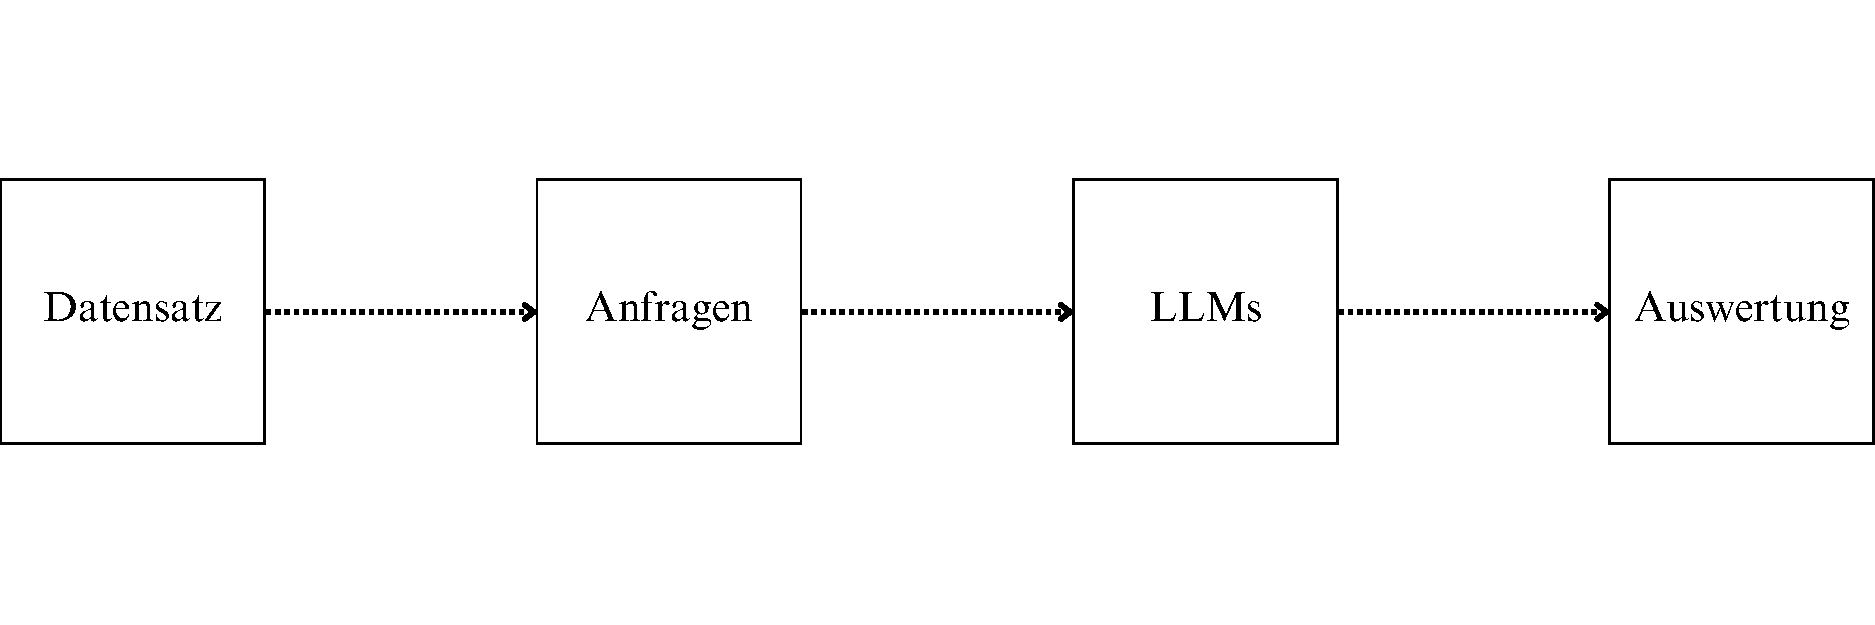
\includegraphics[width=0.95\columnwidth]{img/Ablaufdiagramm.pdf}%
    \caption{Grundstruktur der Experimente.}
    \label{fig_ablauf}
\end{figure}

Zur Beantwortung der Fragestellung werden zwei Experimente durchgeführt.
Im ersten Experiment werden verschiedene Llama 3 Modelle nach den Koordinaten bestimmter Städte befragt.
Die auf diese Weise erhaltenen Antworten werden anschließend mit den tatsächlichen Werten verglichen.
Im zweiten Experiment soll die Distanz zwischen zwei Städten bestimmt werden. Auch diese wird mit der tatsächlichen Distanz verglichen.

Beide Experimente folgen der in Abbildung \ref{fig_ablauf} dargestellten Grundstruktur. Zunächst wird ein passender Datensatz erstellt und daraus entsprechende Anfragen generiert. Diese Anfragen werden an verschiedene LLMs gestellt und die Antworten anschließend für die Analyse aufbereitet, die in Kapitel \ref{ch:results} vorgestellt wird.

Die praktische Umsetzung der Methodik, die gesammelten Daten und die Auswertungen sind zu finden unter: \url{https://github.com/JustusKlameth/ba-dev}.

\section{Koordinaten}
\label{methods_coords}
In diesem Experiment wird der Fokus darauf gelegt zu ermitteln, \textit{in welchem Umfang ausgewählte Llama 3 Modelle in der Lage sind, akkurate Koordinaten für Städte anzugeben}.
Zu diesem Zweck werden die Llama 3 Modelle ähnlich zur Vorgehensweise von \mbox{\citet{bhandariAreLargeLanguage2023}} nach den Koordinaten von Städten befragt und die daraus resultierenden Antworten ausgewertet.

Darüber hinaus werden drei verschiedene Methoden getestet, um die angestrebten Informationen zu erlangen.
Des Weiteren wird untersucht, welchen Einfluss es hat, zusätzlich zum Städtenamen auch das zugehörige Land zu übergeben.

\subsection{Datensatz}
\label{ss:methods:coords:data}
Der Datensatz umfasst die global verteilten 3.527 Städte aus dem MaxMind Datensatz\footnote{\url{https://www.kaggle.com/datasets/max-mind/world-cities-database}} mit mindestens 100.000 Einwohnern.
Dieser Datensatz wurde ausgewählt, weil er alle für die Auswertung relevanten Informationen enthält (Städtename, Ländercode, Längen- und Breitengrad).
Außerdem erlaubt dieser Datensatz einen Vergleich mit den Ergebnissen von \citet{bhandariAreLargeLanguage2023}.

\subsection{Anfragen}
Die Generierung von Anfragen erfolgt unter Anwendung der Vorlagen \ref{fig_template_json} und \ref{fig_template_original}, wobei für \textit{\{location\}} der Städtename eingesetzt wird.
Darüber hinaus besteht die Option, neben dem Städtenamen auch das zugehörige Land zu verwenden.

Für jede Stadt in dem Datensatz werden vier Anfragen erstellt, also für jede Vorlage einmal mit und einmal ohne die Länderinformation.

Die Vorlage \ref{fig_template_original} wurde ausgewählt, da \citet{bhandariAreLargeLanguage2023} auf diese Weise bereits vielversprechende Ergebnisse mit älteren Llama Modellen erzielt haben.
Zusätzlich wurde die Vorlage \ref{fig_template_json} als Kontrast entwickelt, da sie weniger allgemeine Vorgaben enthält, dafür aber ein festes Antwortformat vorschreibt und damit einen neuen Ansatz verfolgt.

\begin{figure}[tb] % json-Vorlage
    \lstinputlisting[language=json]{code/json.json}
    \caption{Diese Vorlage schreibt das \textit{json}-Format für die Antwort vor. Dafür wird nicht explizit (wie bei \ref{fig_template_original}) darauf hingewiesen, keine falschen Informationen zu verbreiten.}
    \label{fig_template_json}
\end{figure}

\begin{figure}[tb] % originale-Vorlage
    \lstinputlisting[language=json]{code/original.json}
    \caption{Vorlage von \citet{bhandariAreLargeLanguage2023}. Diese Vorlage nutzt eine offene Formulierung und schreibt kein Antwortformat vor.}
    \label{fig_template_original}
\end{figure}

\subsection{LLMs}
Mit diesen Anfragen werden das Llama-3.3-70B-Instruct Modell und die Llama-3.1-Instruct Modelle in den Größen 8B, 70B und 405B getestet.
Dafür wird DeepInfra\footnote{\url{https://deepinfra.com/}} genutzt.

Die Llama 3.1 Modelle wurden ausgewählt, da sie die größte Spanne an Parametergrößen innerhalb einer Version liefern und somit einen umfassenden Vergleich ermöglichen.
Das Llama 3.3 Modell wurde zusätzlich betrachtet, um festzustellen, ob es bei gleicher Parameteranzahl eine Verbesserung des geographischen Wissens gibt.

\subsection{Auswertung}
\label{ss:methods:coords:verfahren}
Um die Qualität der Antworten messen zu können, wird als Fehler die geodätische Distanz zwischen den tatsächlichen Koordinaten der Stadt und den Koordinaten der Antwort des LLMs verwendet.
Dafür wird der Algorithmus von \citet{karneyAlgorithmsGeodesics2013} mit dem WGS-84-Ellipsoiden verwendet\footnote{Implementierung: \url{https://geopy.readthedocs.io/en/stable/\#module-geopy.distance}}.

Zur Extraktion der Koordinaten aus der Antwort des LLMs werden drei verschiedene Verfahren genutzt.

Bei der Vorlage \ref{fig_template_json} wird das \textit{json}-Format für die Antwort vorgeschrieben. Demzufolge können die Koordinaten extrahiert werden, indem die Antwort als \textit{json}-Objekt interpretiert wird. Falls dies nicht möglich ist, wird die Antwort als fehlerhaft eingestuft. Diese Art der Auswertung wird im Folgenden als \textit{json} bezeichnet.

Bei der Vorlage \ref{fig_template_original} wird kein Antwortformat vorgeschrieben. Daher sind die Antworten häufig Fließtexte. Um aus diesen Texten die Koordinaten zu extrahieren, werden zwei verschiedene Verfahren angewendet. Das erste Verfahren stammt von \citet{bhandariAreLargeLanguage2023} und wurde unverändert übernommen, um eine Vergleichbarkeit zu ermöglichen\footnote{\url{https://github.com/prabin525/spatial-llm/blob/main/coor-prediction/calculate_errs.py}}. Dieses Verfahren basiert auf regulären Ausdrücken und wird daher im Folgenden als \textit{regex} bezeichnet.

Das zweite Verfahren für Fließtexte liefert einen alternativen Ansatz zur Extraktion der Koordinaten und wurde speziell mit dem Ziel entwickelt, alle möglichen Darstellungen von Koordinaten zu erkennen.
Um dies zu erreichen, wurde das Llama-3.1-8B-Instruct-Turbo Modell mit dem in Abbildung \ref{fig_template_llm} dargestellten System Prompt genutzt und der Fließtext als Nutzereingabe verwendet.
Die dadurch entstehende Antwort wird mit dem \textit{json}-Verfahren weiterverarbeitet, da das System Prompt das \textit{json}-Format vorschreibt.
Dieses Verfahren wird im Folgenden als \textit{llm} bezeichnet.

Des Weiteren ist darauf zu achten, dass für die \textit{regex}- und \textit{llm}-Verfahren stets die Vorlage \ref{fig_template_original} und für das \textit{json}-Verfahren stets die Vorlage \ref{fig_template_json} verwendet wurde.

\begin{figure}[tb]
    \lstinputlisting[language=json]{code/llm.md}
    \caption{System Prompt für das \textit{llm}-Verfahren.}
    \label{fig_template_llm}
\end{figure}

\section{Distanz}
\label{methods_dist}
In diesem Experiment wird der Frage nachgegangen, \textit{in welchem Umfang ausgewählte Llama 3 Modelle in der Lage sind, Distanzen zwischen Städten zu bestimmen}.
Zu diesem Zweck werden die Llama 3 Modelle anhand der im Datensatz enthaltenen Stadt-Paare befragt und die erhaltenen Antworten ausgewertet.

Darüber hinaus wird untersucht, welchen Einfluss die Hinzunahme des Landes auf die Genauigkeit hat.

\subsection{Datensatz}
Um einen geeigneten Datensatz zu erstellen, werden aus dem Datensatz \ref{ss:methods:coords:data} zufällige Paare gebildet. Dadurch entstehen 1.763 Paare von Städten mit mindestens 100.000 Einwohnern.

\subsection{Anfragen}
Die Anfragen werden durch die Anwendung der Vorlage \ref{fig_template_dist} erstellt.
Dafür werden für \textit{\{location\_1\}} und \textit{\{location\_2\}} die jeweiligen Städtenamen eingesetzt.
Außerdem besteht die Möglichkeit, neben den Städtenamen auch die zugehörigen Länder einzusetzen.

Auf diese Weise werden für jedes Stadt-Paar im Datensatz zwei Anfragen erstellt, wobei die erste Anfrage lediglich die Städtenamen und die zweite die Städtenamen sowie die Länder beinhaltet.

Für dieses Experiment wird eine Vorlage zur Erstellung der Anfragen verwendet, die - ähnlich wie Vorlage \ref{fig_template_json} aus dem vorigen Experiment - das \textit{json}-Format vorschreibt.
Diese Entscheidung wurde getroffen, da das \textit{json}-Verfahren praktisch immer auswertbare Antworten produziert und keine zusätzliche intransparente Komponente wie das \textit{llm}-Verfahren einbringt (vgl. Kapitel \ref{ch:results} und \ref{ch:discussion}).

\begin{figure}[tb] % distance-Vorlage
    \lstinputlisting[language=json]{code/json-dist.json}
    \caption{Diese Vorlage schreibt das \textit{json}-Format für die Antwort vor. Außerdem wird die Einheit Kilometer vorgegeben.}
    \label{fig_template_dist}
\end{figure}

\subsection{LLMs}
Wie beim vorigen Experiment, werden mit diesen Anfragen das Llama-3.3-70B-Instruct Modell und die Llama-3.1-Instruct Modelle in den Größen 8B, 70B und 405B getestet.
Dafür wird DeepInfra\footnote{\url{https://deepinfra.com/}} genutzt.

\subsection{Auswertung}
Die Qualität der Antworten wird gemessen, indem der absolute Unterschied zwischen der tatsächlichen geodätischen Distanz (basierend auf den realen Koordinaten der Städte) und der vom LLM angegeben Distanz als Fehler verwendet wird.
Zur Berechnung der geodätischen Distanz wird der Algorithmus von \citet{karneyAlgorithmsGeodesics2013} mit dem WGS-84-Ellipsoiden verwendet\footnote{Implementierung: \url{https://geopy.readthedocs.io/en/stable/\#module-geopy.distance}}.

Zur Extraktion der Distanzen aus den Antworten des LLMs wird genutzt, dass die verwendete Vorlage \ref{fig_template_dist} das \textit{json}-Format für die Antworten vorschreibt. Dementsprechend werden die Antworten als \textit{json}-Objekt interpretiert, sofern dies möglich ist. Andernfalls werden die Antworten als fehlerhaft markiert.

\chapter{Ergebnisse}
\label{ch:results}

\newcommand{\regex}{\textit{regex}}
\newcommand{\llm}{\textit{llm}}
\newcommand{\json}{\textit{json}}

\newcommand{\regexv}{{\regex}-Verfahren}
\newcommand{\llmv}{{\llm}-Verfahren}
\newcommand{\jsonv}{{\json}-Verfahren}

% -------------------------------------------------------------------
% Einleitung
% -------------------------------------------------------------------

% Bezug auf die Fragestellung der Arbeit
In diesem Kapitel werden die Resultate präsentiert, die zur Beantwortung der folgenden Fragestellung dienen:

\begin{center}
    \itshape
    In welchem Umfang sind ausgewählte Llama 3 Modelle in der Lage, akkurate Koordinaten für Städte anzugeben und Distanzen zwischen Städten zu bestimmen?
\end{center}

% Übersicht über das Kapitel
Zunächst werden die Resultate des Experiments \textit{Koordinaten} (\ref{methods_coords}) präsentiert.
Zu diesem Zweck werden zu Beginn die Fehler der verschiedenen Modelle und der verschiedenen Vorlagen ohne die Länderinformation quantitativ miteinander verglichen.
Im Anschluss daran wird erörtert, welchen Einfluss die Hinzunahme des Landes hat.
Abschließend werden qualitative Beispiele vorgestellt und häufige Fehler und Probleme präsentiert.

Im weiteren Verlauf werden die Resultate des Experiments \textit{Distanz} (\ref{methods_dist}) dargestellt.
Für dieses Experiment erfolgt ebenso zunächst eine quantitative Analyse der Fehler der verschiedenen Modelle und der verschiedenen Vorlagen ohne Länderinformation.
Im Anschluss daran wird der Einfluss der Länderinformation untersucht.
Schließlich werden qualitative Beispiele vorgestellt und häufige Fehler und Probleme illustriert.

% -------------------------------------------------------------------
% Inhalt: Koordinaten
% -------------------------------------------------------------------
\section{Koordinaten}
\label{results_coords}
% Einleitung: Was wird gemacht?
Im Folgenden werden die Ergebnisse des Experiments \textit{Koordinaten} dargestellt, die aus der in Kapitel \ref{methods_coords} beschriebenen Vorgehensweise resultieren.

\subsection{Quantitativer Vergleich der verschiedenen LLMs und Verfahren}
% Allg. Informationen zur Auswertung
Bei den Auswertungen und Visualisierungen in diesem Kapitel wird häufig der durchschnittliche Fehler dargestellt.
Damit ist der durchschnittliche Fehler aller Antworten gemeint, die die angegebenen Bedingungen erfüllen, d.\,h. z.\,B. alle Antworten des Llama-3.3-70B-Instruct Modells mit dem \jsonv{} und den Länderinformationen.
Dabei werden die fehlerhaften Antworten der LLMs nicht berücksichtigt.

\subsubsection*{Ohne die Länderinformation}

\begin{figure}[tb] % Fehler der Modelle mit den Verfahren (ohne Land)
    \centering
    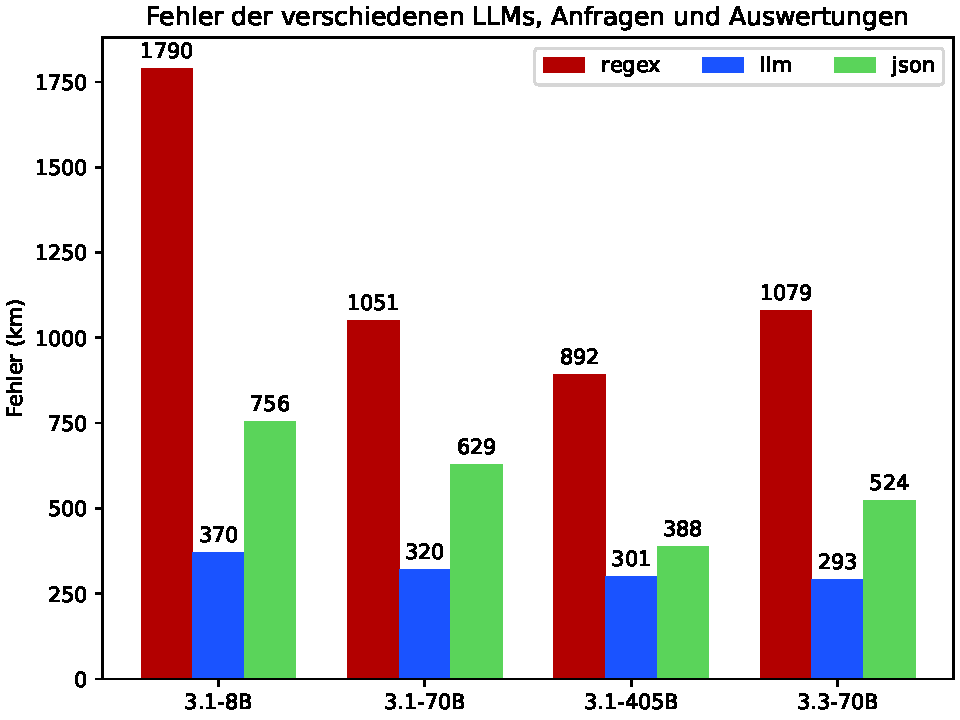
\includegraphics[width=0.7\columnwidth]{img/size_template_error_no_std.pdf}
    \caption{Der durchschnittliche Fehler von den verschiedenen LLMs, Anfragen und Auswertungsverfahren ohne die Länderinformation für das Experiment \textit{Koordinaten} (\ref{methods_coords}). Dabei werden die Fehler für die LLMs Llama-3.1-Instruct in den Größen 8B, 70B, 405B und Llama-3.3-70B-Instruct (links nach rechts) für jeweils die Auswertungsverfahren \regex{} (rot), \llm{} (blau) und \json{} (grün) mit den zugehörigen Vorlagen visualisiert.}
    \label{fig_res_coords_error}
\end{figure}

% Reihenfolge: regex > json > llm
Der durchschnittliche Fehler der Anfragen ohne zusätzliche Länderinformationen zeigt, dass für alle betrachteten Modelle das \llmv{} am besten und das \regexv{} am schlechtesten ist, während das \jsonv{} zwischen den beiden anderen liegt.
Dabei fällt auf, dass der Abstand zwischen dem \regex{}- und dem \jsonv{} größer ist als zwischen dem \llm{}- und dem \jsonv{} (vgl. Abbildung \ref{fig_res_coords_error}).

% Größe ist gut
Außerdem zeigt die Abbildung \ref{fig_res_coords_error}, dass für alle betrachteten Verfahren die Genauigkeit bei größeren Modellen zunimmt.
Die einzige Ausnahme stellt das Llama-3.3-70B-Instruct Modell mit dem \llmv{} dar, welches für dieses Verfahren die besten Ergebnisse liefert.

\begin{figure}[tb] % p-Werte für ohne Land
    \centering
    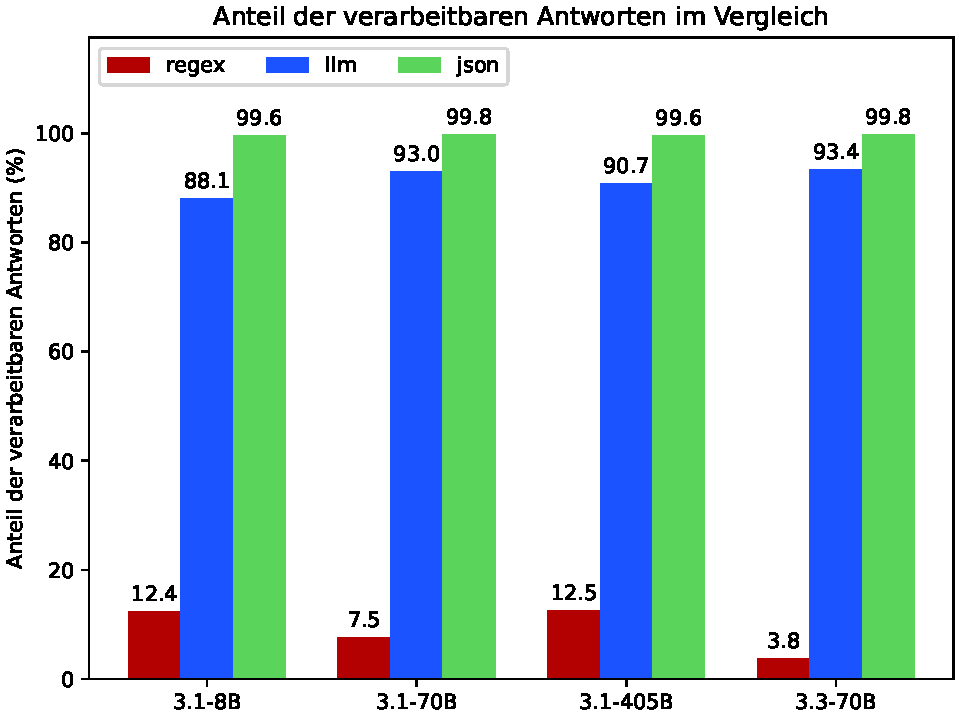
\includegraphics[width=0.7\columnwidth]{img/size_template_p.pdf}
    \caption{Der Anteil der korrekt verarbeitbaren Antworten der verschiedenen LLMs, Anfragen und Auswertungsverfahren für das Experiment \textit{Koordinaten} (\ref{methods_coords}) ohne die Länderinformationen. Dabei werden die Anteile der Antworten, die korrekt verarbeitet werden können, von den LLMs Llama-3.1-Instruct in den Größen 8B, 70B, 405B und Llama-3.3-70B-Instruct (links nach rechts) für jeweils die Auswertungsverfahren \regex{} (rot), \llm{} (blau) und \json{} (grün) mit den zugehörigen Vorlagen visualisiert.}
    \label{fig_res_coords_p}
\end{figure}

% p-Wert
% ----------------
% regex: 9.04 3.63
% llm: 91.3 2.1
% json: 99.7 0.09
% ----------------
Der Anteil der verarbeitbaren Antworten für die Anfragen ohne Länderinformationen (vgl. Abbildung \ref{fig_res_coords_p}) zeigt, dass die Verfahren unabhängig vom Modell relativ konstante Fehlerraten aufweisen.
Die Mittelwerte betragen für das \regexv{} \( \num{9.04} \pm \num{3.63} \), für das \llmv{} \( \num{91.3} \pm \num{2.1} \) und für das \jsonv{} \( \num{99.7} \pm \num{0.09} \).
Dabei fällt auf, dass das \jsonv{} nahezu fehlerfrei ist, während das \regexv{} im Durchschnitt über 90 Prozent der Anfragen so fehlerhaft beantwortet, dass es nicht möglich ist, Koordinaten zu extrahieren.

% p-Werte und Fehler passen gut zusammen
Die in den Abbildungen \ref{fig_res_coords_error} und \ref{fig_res_coords_p} dargestellten Ergebnisse weisen beide ein Muster auf.
Bei jedem Modell hat das \regexv{} eindeutig den größten durchschnittlichen Fehler und bei weitem die meisten fehlerhaften Antworten.
Im Kontrast dazu liegen das \json{}- und das \llmv{} deutlich näher beieinander.
Das \llmv{} liefert etwas bessere durchschnittliche Fehler, dafür das \jsonv{} aber nahezu keine fehlerhaften Antworten.

% Begründung: Name der Städte ist nicht eindeutig
Allerdings entstehen bei diesem Verfahren teilweise große Fehler für einzelne Städte.
Dies liegt unter anderem daran, dass Städtenamen nicht eindeutig sind.
Das führt dazu, dass Koordinaten für andere Städte mit dem gleichen Namen zurückgegeben werden.
Dies könnte der Grund dafür sein, dass z.\,B. bei dem Llama-3.1-405B-Instruct Modell mit dem \jsonv{} ohne die Länderinformation unter 1 {\%} der Anfragen für über 35 {\%} des Gesamtfehlers verantwortlich sind.
In der Abbildung \ref{fig_res_muenster_total} ist z.\,B. dargestellt, dass bei diesen Anfragen die Stadt Münster (NRW, Deutschland) wahrscheinlich mit der südlichsten Provinz Munster in Irland\footnote{\url{https://de.wikipedia.org/wiki/Munster_(Irland)}} verwechselt wurde.

\subsubsection*{Mit der Länderinformation}
Daher wird im Folgenden vorgestellt, was passiert, wenn das Land zu den Anfragen hinzugefügt wird.

\begin{figure}[tb] % Fehler der Modelle mit den Verfahren (mit Land)
    \centering
    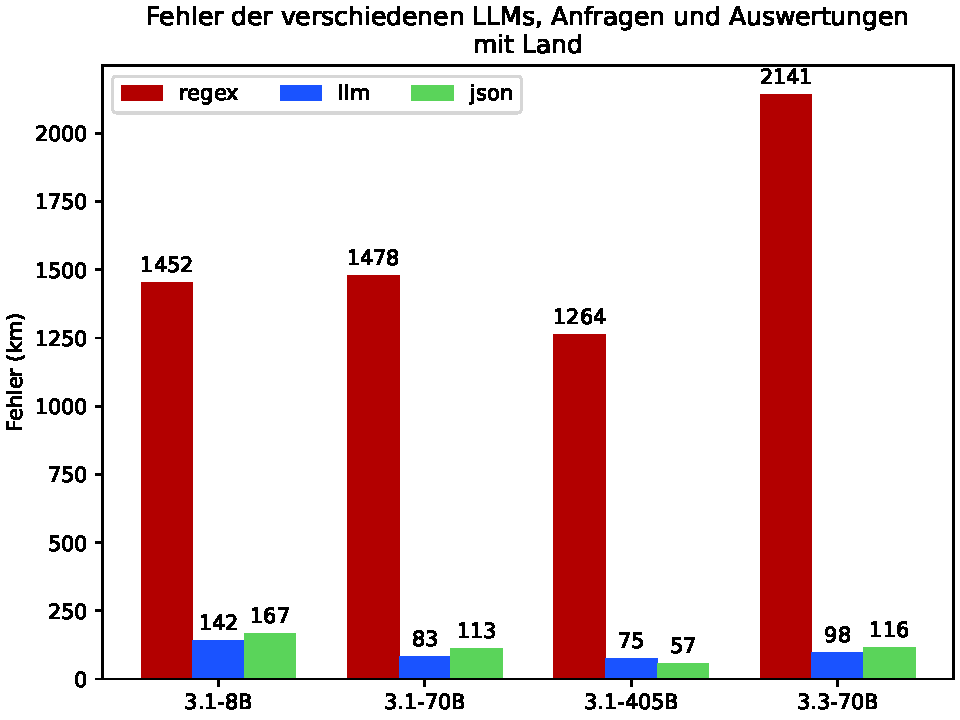
\includegraphics[width=0.7\columnwidth]{img/country_error_no_std.pdf}
    \caption{Der durchschnittliche Fehler von den verschiedenen LLMs, Anfragen und Auswertungsverfahren mit der Länderinformation für das Experiment \textit{Koordinaten} (\ref{methods_coords}). Dabei werden die Fehler für die LLMs Llama-3.1-Instruct in den Größen 8B, 70B, 405B und Llama-3.3-70B-Instruct (links nach rechts) für jeweils die Auswertungsverfahren \regex{} (rot), \llm{} (blau) und \json{} (grün) mit den zugehörigen Vorlagen visualisiert.}
    \label{fig_res_coords_error_country}
\end{figure}

% regex > json > llm
Der durchschnittliche Fehler der Anfragen mit der Länderinformation (vgl. Abbildung \ref{fig_res_coords_error_country}) zeigt ein ähnliches Muster wie der durchschnittliche Fehler der Anfragen ohne die Länderinformationen (vgl. Abbildung \ref{fig_res_coords_error}).
Bei beiden Arten der Anfragen ist das \regexv{} am schlechtesten, wobei der Abstand bei den Anfragen mit der Länderinformation deutlich angestiegen ist.
Außerdem schneidet bei beiden das \llmv{} am besten ab und das \jsonv{} liegt in der Mitte.
Ein Ausreißer sind die Anfragen mit der Länderinformation für das Llama-3.1-405B-Instruct Modell.
Hier liefert das \jsonv{} etwas bessere Ergebnisse als das \llmv{}.

% Größe ist gut, außer bei regex
Außerdem zeigt die Abbildung \ref{fig_res_coords_error_country}, dass bei den \json{}- und \llmv{} die Genauigkeit der Antworten für größere Modelle zunimmt.

\begin{figure}[tb] % p-Werte für mit Land
    \centering
    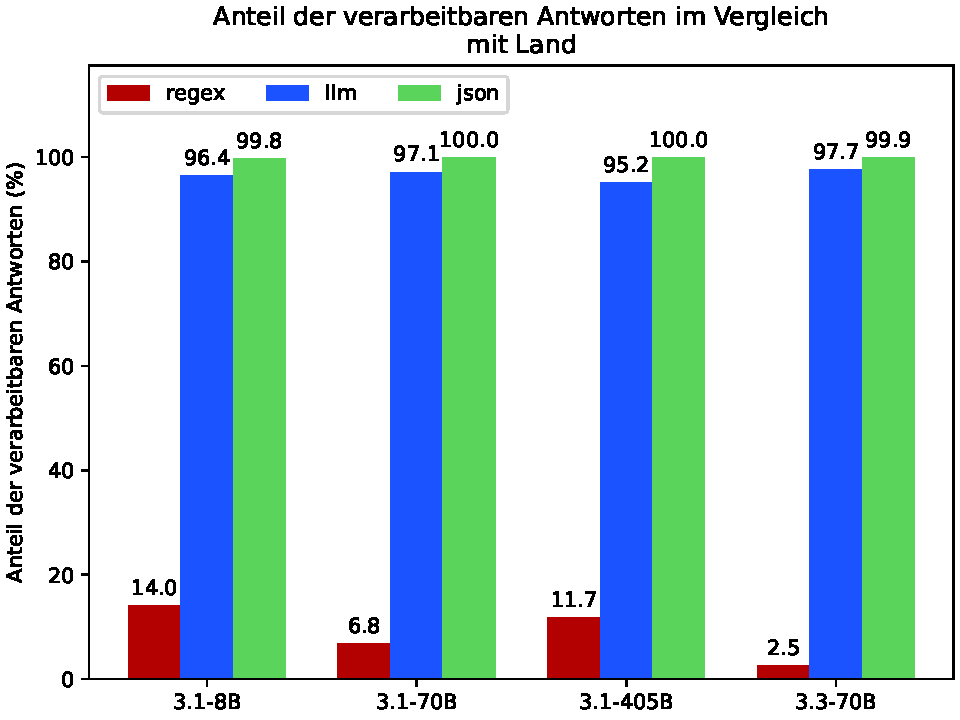
\includegraphics[width=0.7\columnwidth]{img/country_p.pdf}
    \caption{Der Anteil der korrekt verarbeitbaren Antworten der verschiedenen LLMs, Anfragen und Auswertungsverfahren für das Experiment \textit{Koordinaten} (\ref{methods_coords}) mit der Länderinformation. Dabei werden die Anteile der Antworten, die korrekt verarbeitet werden können, von den LLMs Llama-3.1-Instruct in den Größen 8B, 70B, 405B und Llama-3.3-70B-Instruct (links nach rechts) für jeweils die Auswertungsverfahren \regex{} (rot), \llm{} (blau) und \json{} (grün) mit den zugehörigen Vorlagen visualisiert.}
    \label{fig_res_coords_p_country}
\end{figure}

% p-Wert
% ----------------
% regex: 8.76 4.46
% llm: 96.6 0.95
% json: 99.91 0.09
% ----------------
Der Anteil der verarbeitbaren Antworten verändert sich durch die Hinzunahme der Länderinformation kaum (vgl. Abbildungen \ref{fig_res_coords_p} und \ref{fig_res_coords_p_country}).
Dabei bleiben die Fehlerraten für die verschiedenen Verfahren unabhängig von der Modellgröße relativ konstant; das \regexv{} sehr fehleranfällig, das \llmv{} sehr gut und das \jsonv{} praktisch perfekt.
Die Mittelwerte betragen für das \regexv{} \( \num{8.76} \pm \num{4.46} \), für das \llmv{} \( \num{96.6} \pm \num{0.95} \) und für das \jsonv{} \( \num{99.91} \pm \num{0.09} \).

% p-Werte und Fehler passen gut zusammen?
Durch Hinzunahme des Landes bei den Anfragen ändert sich nicht, dass das \regexv{} den größten Fehler und mit Abstand die wenigsten zulässigen Antworten produziert und die beiden anderen Verfahren relativ nah beisammen sind.

\subsubsection*{Auswirkungen der Hinzunahme der Länderinformation}

\begin{figure}[tb] % country vs. no country
    \centering
    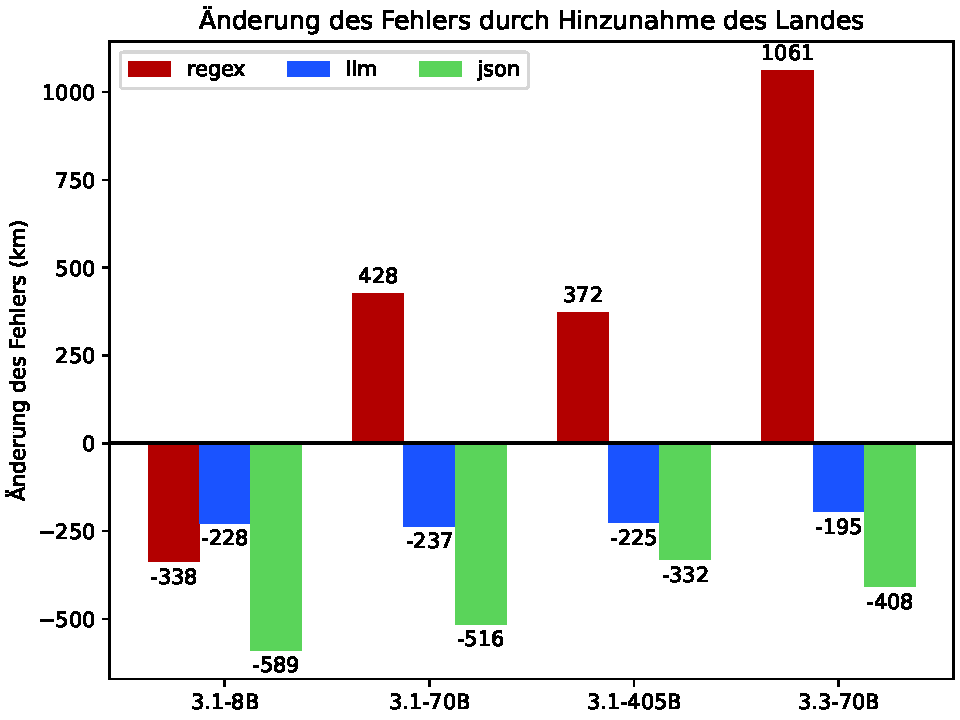
\includegraphics[width=0.7\columnwidth]{img/country_vs_no_country.pdf}
    \caption{Die Differenz zwischen den in den Abbildungen \ref{fig_res_coords_error} und \ref{fig_res_coords_error_country} dargestellten Ergebnissen des Experiments \textit{Koordinaten} (\ref{methods_coords}). Dadurch wird der Einfluss der Länderinformation in den Anfragen dargestellt. Ein negativer Wert bedeutet in dem Fall, dass der Fehler durch die Hinzunahme der Länderinformation um diesen Wert kleiner geworden ist.}
    \label{fig_res_coords_country}
\end{figure}

% -------------------------------------------------------------
% regex: \( \SI{-40.48}{\percent} \pm \num{41.45} \) Prozentpunkte
% llm: \( \SI{69.27}{\percent} \pm \num{5.49} \) Prozentpunkte
% json: \( \SI{80.83}{\percent} \pm \num{3.15} \) Prozentpunkte
% -------------------------------------------------------------

% Differenz
Die Differenz zwischen den Ergebnissen des Experiments \textit{Koordinaten} (\ref{methods_coords}) ohne die Länderinformation (vgl. Abbildung \ref{fig_res_coords_error}) und mit der Länderinformation (vgl. Abbildung \ref{fig_res_coords_error_country}) ist in der Abbildung \ref{fig_res_coords_country} dargestellt.
Anhand der Abbildung lässt sich erkennen, dass die Länderinformation keine einheitliche und tendenziell eine verschlechternde Wirkung auf das \regexv{} hat.
Bei den anderen beiden Verfahren werden die Ergebnisse durch die Hinzunahme des Landes für jedes Modell besser.
Dabei fällt auf, dass die Verbesserung für das \jsonv{} bei jedem Modell größer ist, als beim \llmv{}.
Das sorgt dafür, dass die Differenz der Fehler der \json{}- und \llmv{} nach Hinzunahme der Länderinformation deutlich kleiner geworden ist (vgl. Abbildungen \ref{fig_res_coords_error} und \ref{fig_res_coords_error_country}).

\subsubsection*{Standardabweichung}
Allerdings fällt auf, dass die Standardabweichung für alle Modelle und alle Anfragearten sehr hoch ist und sich relativ zum durchschnittlichen Fehler durch die Hinzunahme der Länderinformation kaum ändert (vgl. Abbildung \ref{fig_std_total}).

\begin{figure} % Fehler mit und ohne Länderinformation mit std
    \centering
    \begin{subfigure}{.5\textwidth}
      \centering
      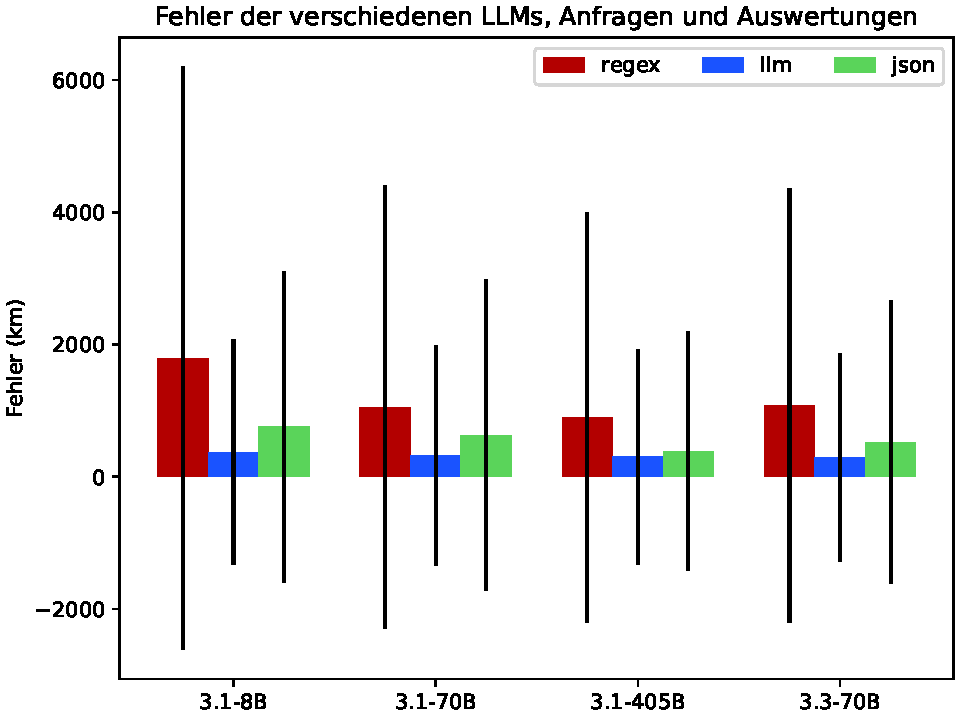
\includegraphics[width=.95\linewidth]{img/size_template_error.pdf}
      \caption{Ohne die Länderinformation.}
      \label{fig_std_without_country}
    \end{subfigure}%
    \begin{subfigure}{.5\textwidth}
      \centering
      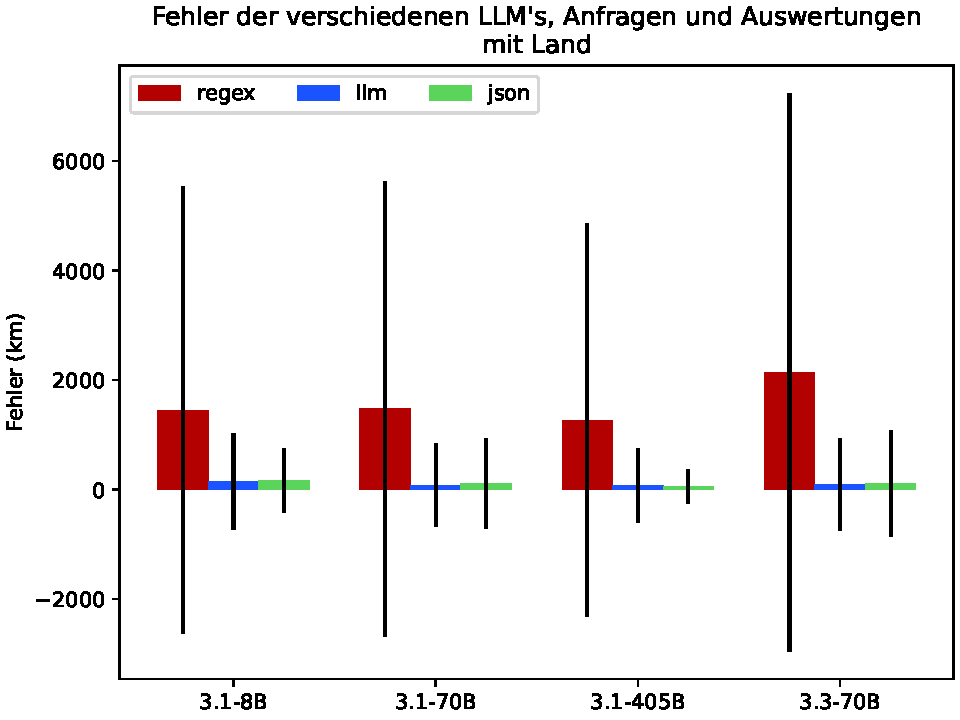
\includegraphics[width=.95\linewidth]{img/country_error.pdf}
      \caption{Mit der Länderinformation.}
      \label{fig_std_with_country}
    \end{subfigure}
    \caption{Der durchschnittliche Fehler von den verschiedenen LLMs, Anfragen und Auswertungsverfahren einmal mit und einmal ohne die Länderinformation für das Experiment \textit{Koordinaten} (\ref{methods_coords}). Dabei werden die Fehler für die LLMs Llama-3.1-Instruct in den Größen 8B, 70B, 405B und Llama-3.3-70B-Instruct (links nach rechts) für jeweils die Auswertungsverfahren \regex{} (rot), \llm{} (blau) und \json{} (grün) mit den zugehörigen Vorlagen visualisiert. Zusätzlich wird außerdem die Standardabweichung für jeden Anfragetypen in schwarz visualisiert.}
    \label{fig_std_total}
\end{figure}

\subsection{Qualitative Beispiele und Erörterung}
Im Folgenden werden einzelne Anfragen qualitativ genauer betrachtet, um das Verhalten der LLMs bei den verschiedenen Anfragearten und häufige Fehler darzustellen.

Für die Unterkapitel \textit{Ablauf und Probleme} der verschiedenen Verfahren wird das Llama-3.1-8B-Instruct Modell mit Anfragen für Abu Dhabi ohne die Länderinformation genutzt.
Außerdem werden die in Kapitel \ref{ch:methods} beschriebenen System Prompts und Vorlagen genutzt, um die Anfragen zu generieren.

\subsubsection*{Ablauf und Probleme: \regexv{}}
% Normaler Ablauf bei regex
Bei dem \regexv{} wird eine Vorlage verwendet, die kein Antwortformat vorschreibt (vgl. Abbildung \ref{fig_template_original}).
Dadurch entsteht die längere Antwort \ref{answer_original}. Trotz der Tatsache, dass die Antwort offensichtlich Koordinaten enthält, schafft es das \regexv{} nicht, Koordinaten zu extrahieren und damit einen Fehler zu berechnen.
Das kommt sehr häufig vor\footnote{Da das \regex{}- und \llmv{} dieselben Antworten auswerten, ist dies an dem Anteil der verarbeitbaren Antworten (s. Abbildung \ref{fig_res_coords_p}) erkennbar.}.

Dies ist auch das Hauptproblem des \regexv{}s.
Da aus sehr vielen Antworten fehlerhafterweise keine Koordinaten extrahiert werden, ist es nicht möglich, zuverlässige Werte zu erhalten.

\begin{figure} % Antwort für originales Template

    \begin{lstlisting}[literate={°}{\textdegree}1, breaklines=true]
        The coordinates of Abu Dhabi, the capital city of the United Arab Emirates, are:

        Latitude: 24.4653° N
        Longitude: 54.3703° E

        Please note that these coordinates are for the city center of Abu Dhabi. If you need the coordinates for a specific location within the city or the emirate, please let me know and I'll do my best to provide you with the accurate information.
    \end{lstlisting}

    \caption{Die Antwort des Llama-3.1-8B-Instruct Modells auf die Anfrage für Abu Dhabi ohne die Länderinformation mit der Vorlage \ref{fig_template_original}.}

    \label{answer_original}
\end{figure}

\subsubsection*{Ablauf und Probleme: \llmv{}}
% Normaler Ablauf bei llm
Auch das \llmv{} wertet die Antwort \ref{answer_original} aus.
Dafür wird, wie in Kapitel \ref{ch:methods} beschrieben, eine Anfrage an das Llama-3.1-8B-Instruct-Turbo Modell mit dem System Prompt \ref{fig_template_llm} und der vorigen Antwort \ref{answer_original} als Nutzereingabe gesendet.
Dabei entsteht die Antwort \ref{answer_llm}.
Diese Antwort kann sehr zuverlässig mit dem \jsonv{} ausgewertet werden.

Dabei ist das Hauptproblem, dass beim Extrahieren der Koordinaten ein anderes LLM verwendet wird.
Es kann nicht ausgeschlossen werden, dass dieses Modell fehlerhafte Koordinaten durch bessere ersetzt oder sogar bei Antworten, die keine Koordinaten enthalten, Koordinaten hinzufügt.
Allerdings zeigen die durchschnittlichen Fehler für das \llmv{} (vgl. Abbildung \ref{fig_res_coords_error}), dass das Llama-3.1-8B-Instruct Modell den größten Fehler hat.
Das lässt vermuten, dass das Llama-3.1-8B-Instruct-Turbo Modell, falls es nicht nur Koordinaten extrahieren sollte, das Ergebnis wahrscheinlich verschlechtert und nicht verbessert.

\begin{figure} % Antwort für llm-Verfahren (praktisch json-Template)

    \begin{lstlisting}[literate={°}{\textdegree}1, breaklines=true]
        {""latitude"": ""24.4653"", ""longitude"": ""54.3703""}
    \end{lstlisting}

    \caption{Die Antwort des Llama-3.1-8B-Instruct-Turbo Modells auf die Anfrage des \llmv{}s für die vorige Antwort \ref{answer_original}.}

    \label{answer_llm}
\end{figure}

\subsubsection*{Ablauf und Probleme: \jsonv{}}
% Normaler Ablauf bei json
Das \jsonv{} verwendet die Vorlage \ref{fig_template_json} und schreibt damit, genau wie die zweite Anfrage des \llmv{}s, ein festes Antwortformat vor.
Dadurch entsteht die zu der Antwort \ref{answer_llm} sehr ähnliche Antwort \ref{answer_json}.
Diese Antwort wird dann direkt ausgewertet (wie in Kapitel \ref{ch:methods} beschrieben) und der Fehler berechnet.

Dabei gibt es keine häufig auftretenden Probleme, die mit dem Verfahren zusammenhängen.

\begin{figure} % Antwort für das json-Verfahren

    \begin{lstlisting}
        {""latitude"": 24.465646, ""longitude"": 54.369824}
    \end{lstlisting}

    \caption{Die Antwort des Llama-3.1-8B-Instruct Modells auf die Anfrage für Abu Dhabi ohne die Länderinformation mit der Vorlage \ref{fig_template_json}.}

    \label{answer_json}
\end{figure}

\subsubsection*{Gleiche Städte- oder Regionennamen}
% Problem: Gleiche Städtenamen
Ein häufig auftretendes Problem ist, dass der Name einer Stadt oder Region nicht eindeutig ist, weil er z.\,B. in verschiedenen Ländern verwendet wird.
Das führt zu besonders großen Fehlern, da das LLM nur anhand des Städtenamens nicht zwischen gleichnamigen Städten unterscheiden kann und eventuell die Koordinaten einer Stadt auf einem anderen Kontinent zurückgibt, die aber nicht gemeint ist.

In Abbildung \ref{fig_res_muenster_total} wird visualisiert, dass diese Verwechselung mit dem Llama-3.1-405B-Instruct Modell bei dem \jsonv{} für die Stadt Münster (NRW, Deutschland) passiert ist.
Außerdem ist dargestellt, dass durch die Hinzunahme des Landes die Verwechselung verhindert wurde.

\begin{figure} % Karten mit Münster
    \centering
    \begin{subfigure}{.5\textwidth}
      \centering
      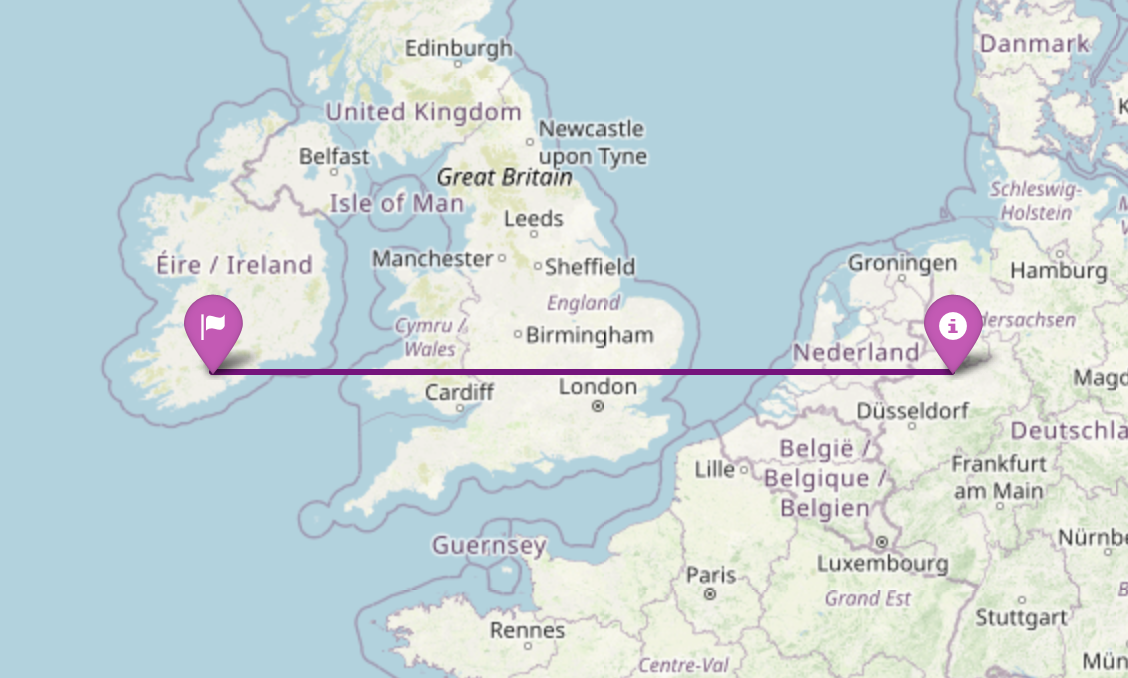
\includegraphics[width=.95\linewidth]{img/Karte-Muenster.png}
      \caption{Ohne die Länderinformation.}
      \label{fig_res_muenster}
    \end{subfigure}%
    \begin{subfigure}{.5\textwidth}
      \centering
      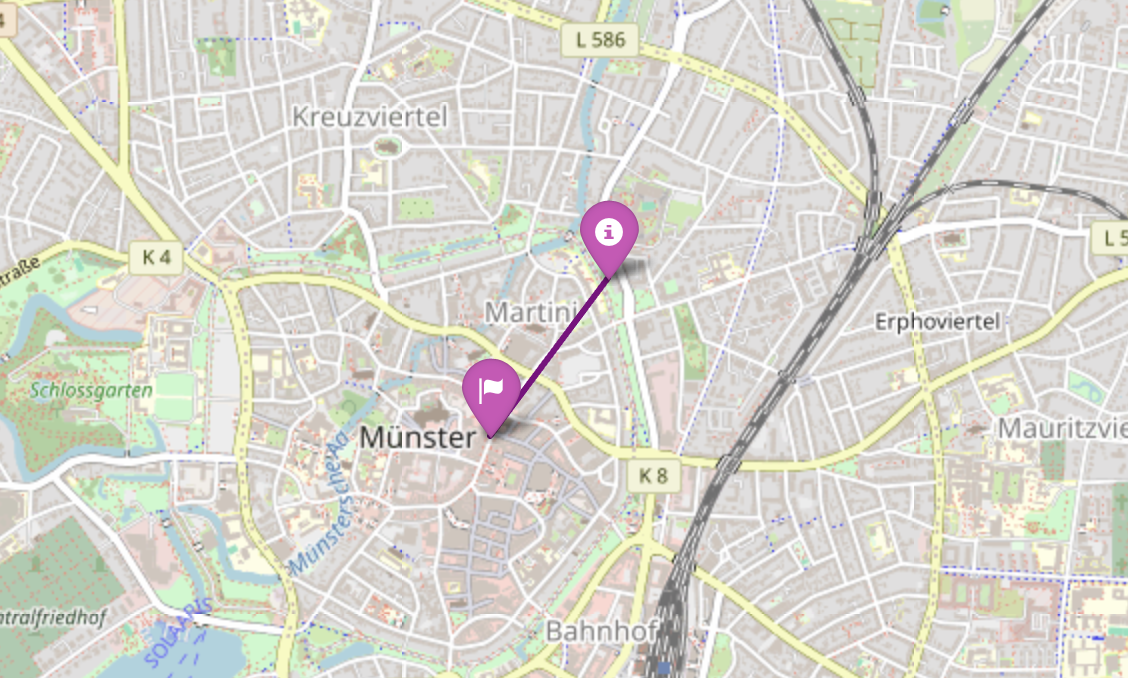
\includegraphics[width=.95\linewidth]{img/Karte-Muenster-country.png}
      \caption{Mit der Länderinformation.}
      \label{fig_res_muenster_country}
    \end{subfigure}
    \caption{Die tatsächliche Position der Stadt Münster (NRW, Deutschland) und die Ergebnisse für das Experiment \textit{Koordinaten} (\ref{methods_coords}) von dem Llama-3.1-405B-Instruct Modell mit dem \jsonv{}. Dabei wird visualisiert, welchen Einfluss die Länderinformation für die zurückgegebenen Koordinaten von Münster hat.}
    \label{fig_res_muenster_total}
\end{figure}

% Problem: Gleiche Städtenamen in einem Land
Allerdings werden dadurch nicht alle Verwechselungsprobleme gelöst.
Es kann auch vorkommen, dass innerhalb eines Landes der gleiche Städtename mehrmals verwendet wird.
Das ist für den Gesamtfehler vor allem bei großen Ländern problematisch.
In der Abbildung \ref{fig_pasadena} wird dargestellt, wie das Llama-3.1-8B-Instruct Modell mit dem \jsonv{} trotz der Länderinformation die Koordinaten für Pasadena, Kalifornien\footnote{\url{https://de.wikipedia.org/wiki/Pasadena_(Kalifornien)}} zurückgibt, obwohl Pasadena, Texas\footnote{\url{https://de.wikipedia.org/wiki/Pasadena_(Texas)}} gemeint ist.
Dadurch entsteht ein Fehler von über 2.200 km, der bei einem Durchschnittsfehler für diese Anfragen von ca. 167 km durchaus relevant ist (vgl. Abbildung \ref{fig_res_coords_error_country}).

\begin{figure}[tb] % Karte Pasadena
    \centering
    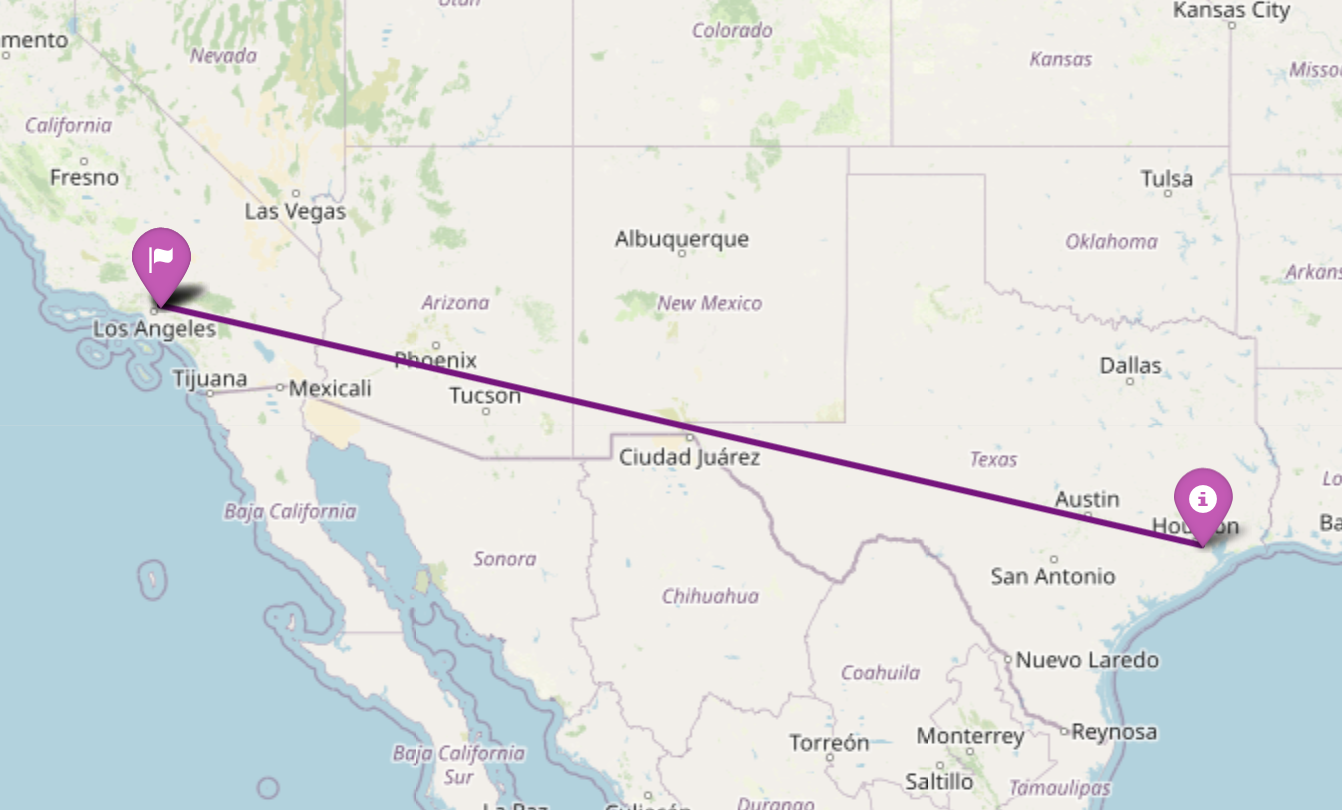
\includegraphics[width=0.7\columnwidth]{img/Karte-Pasadena.png}
    \caption{Das Llama-3.1-8B-Instruct Modell gibt mit dem \jsonv{} trotz der Länderinformation die Koordinaten für Pasadena, Kalifornien zurück, obwohl Pasadena, Texas gemeint ist.}
    \label{fig_pasadena}
\end{figure}

% -------------------------------------------------------------------
% Inhalt: Distanz
% -------------------------------------------------------------------
\section{Distanz}
\label{results_dist}
% Einleitung: Was wird gemacht?
In diesem Abschnitt werden die Resultate des Experiments \textit{Distanz} dargestellt.
Diese basieren auf der in Kapitel \ref{methods_dist} beschriebenen Vorgehensweise.

\subsection{Quantitativer Vergleich der verschiedenen LLMs}
% Was ist der Fehler
Wie bei dem vorigen Experiment wird bei den Auswertungen und Visualisierungen in diesem Kapitel meistens der durchschnittliche Fehler genutzt.
Damit ist der durchschnittliche Fehler aller Antworten gemeint, die die angegebenen Bedingungen erfüllen.
Der einzelne Fehler wird, wie in Kapitel \ref{methods_dist} beschrieben, berechnet.

\begin{figure}[tb] % Fehler Distanz mit und ohne Länderinformation
    \centering
    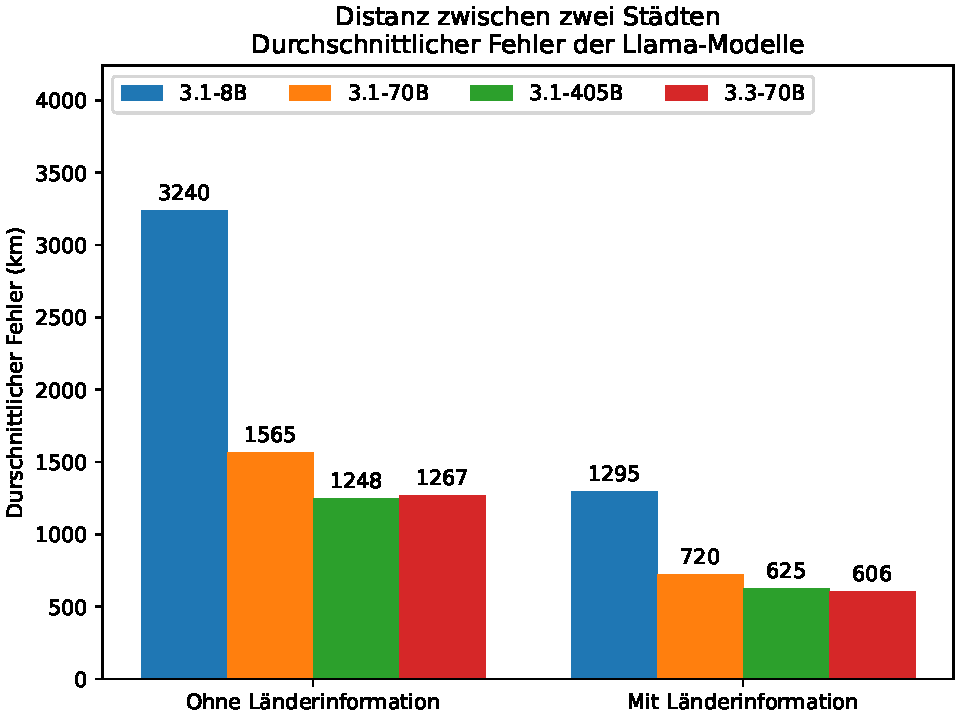
\includegraphics[width=0.7\columnwidth]{img/distance_error.pdf}
    
    \caption{
        Der durchschnittliche Fehler von den verschiedenen LLMs mit und ohne die Länderinformation für das Experiment \textit{Distanz} (\ref{methods_dist}).
        Dabei werden die Fehler für die LLMs Llama-3.1-Instruct in den Größen 8B (blau), 70B (orange), 405B (grün) und Llama-3.3-70B-Instruct (rot) einmal mit (rechts) und einmal ohne (links) die Länderinformation visualisiert.
    }

    \label{fig_dist_error}
\end{figure}

\subsubsection*{Ohne die Länderinformation}
Die durchschnittlichen Fehler ohne die Länderinformation zeigen: Je größer das LLM, desto besser das Ergebnis.
Allerdings ist der Unterschied zwischen dem Llama-3.3-70B-Instruct Modell und dem Llama-3.1-405B-Instruct Modell sehr klein (vgl. Abbildung \ref{fig_dist_error}).

\subsubsection*{Mit der Länderinformation}
Auch bei den durchschnittlichen Fehlern mit der Länderinformation zeigt sich, dass größere Modelle meistens bessere Ergebnisse produzieren (vgl. Abbildung \ref{fig_dist_error}).
Allerdings liefert das Llama-3.3-70B-Instruct Modell die besten Ergebnisse, obwohl es nicht das größte Modell ist.
Dabei muss dennoch beachtet werden, dass hier die älteren Llama 3.1 Modelle\footnote{\url{https://www.llama.com/docs/model-cards-and-prompt-formats/llama3_1/}} mit dem neueren Llama 3.3 Modell\footnote{\url{https://www.llama.com/docs/model-cards-and-prompt-formats/llama3_3/}} verglichen werden.

\subsubsection*{Auswirkungen der Hinzunahme der Länderinformation}
In Abbildung \ref{fig_dist_error} ist gut erkennbar, dass sich der Fehler durch die Hinzunahme der Länderinformation für alle Modelle ungefähr halbiert.
Dazu passt, dass sich beim Experiment \textit{Koordinaten} der Fehler für das \jsonv{} durch Hinzunahme der Länderinformation deutlich verbessert hat.

\subsubsection*{Anteil der verarbeitbaren Antworten}
% p-Werte

\begin{figure}[tb] % Distanz: p-Werte
    \centering
    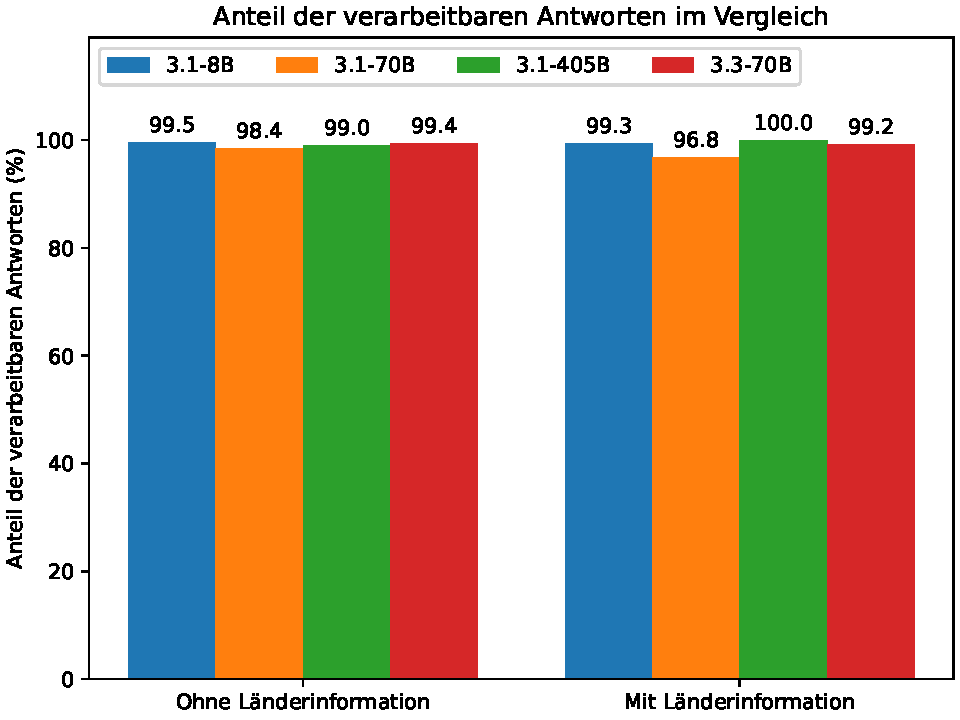
\includegraphics[width=0.7\columnwidth]{img/distance_p.pdf}
    
    \caption{
        Der Anteil der korrekt verarbeitbaren Antworten der verschiedenen LLMs mit und ohne die Länderinformation für das Experiment \textit{Distanz} (\ref{methods_dist}).
        Dabei werden die Anteile der Antworten, die korrekt verarbeitet werden können, von den LLMs Llama-3.1-Instruct in den Größen 8B (blau), 70B (orange), 405B (grün) und Llama-3.3-70B-Instruct (rot) einmal mit (rechts) und einmal ohne (links) die Länderinformation visualisiert.
    }

    \label{fig_dist_p}
\end{figure}

% ------------------------------
% Original: 99.06 +/- 0.42
% Country: 98.82 +/- 1.23
% ------------------------------

Der Anteil der verarbeitbaren Antworten ist für alle LLMs sehr groß und es gibt keine signifikanten Unterschiede (vgl. Abbildung \ref{fig_dist_p}).
Die Mittelwerte betragen für die Antworten ohne die Länderinformation \( \num{99.06} \pm \num{0.42} \) und für die Antworten mit der Länderinformation \( \num{98.82} \pm \num{1.23} \).
Diese Ergebnisse stimmen mit den nahezu perfekten Antwortraten des \jsonv{}s beim Experiment \textit{Koordinaten} überein.

\subsubsection*{Standardabweichung}
Allerdings fällt auch bei diesem Experiment auf, dass die Standardabweichung für alle Modelle sehr hoch ist.
Die Hinzunahme der Länderinformation verringert die Standardabweichung deutlich.
Trotzdem liegt die geringste Standardabweichung aller LLMs, die vom Llama-3.3-70B Modell erreicht wird, bei ca. 616 km.

\subsection{Qualitative Beispiele und Erörterung}
% Qualitativ: normale Beipsiele, Fehler (Land vs. kein Land, trotz Land falsche Stadt)
Im Folgenden wird eine einzelne Anfrage etwas genauer vorgestellt und auf Probleme eingegangen, um die Ergebnisse und die Vorgehensweise nachvollziehbarer zu machen.

\subsubsection*{Beispiel-Anfrage}
% -------------------------------------------------------------------------------------------------------
% /dev/distance-prediction/answers/llama-3.1-8B-Instruct-json-country.csv
% in,bharuch,153538,21.7,72.966667,de,berlin,3398362,52.516667000000005,13.4,6073.0307874846,"[{'role': 'system', 'content': 'Answer in json format only: {""distance"": < e.g. ""1945.399479"" >}. The value must be in kilometers and no explanation, just the answer!'}, {'role': 'user', 'content': 'What is the distance between bharuch, India and berlin, Germany?'}]","{""distance"": 6171.479892}"
% -------------------------------------------------------------------------------------------------------
Es wird die Anfrage für Bharuch, Indien und Berlin, Deutschland betrachtet.
Mithilfe der Vorlage \ref{fig_template_dist} und der Länderinformation wird die Anfrage \ref{dist_message} erstellt.
Die Antwort des Llama-3.1-8B-Instruct Modells auf diese Anfrage ist in der Abbildung \ref{dist_answer} dargestellt und entspricht einer Standardantwort für das \jsonv{}.
Mit dieser Antwort kann die Distanz direkt extrahiert werden.
In diesem Beispiel beträgt der Fehler ca. 100 km.

\begin{figure} % Anfrage für distance

    \begin{lstlisting}[literate={°}{\textdegree}1, breaklines=true]
        [
            {
                'role': 'system',
                'content': 'Answer in json format only: {""distance"": < e.g. ""1945.399479"" >}. The value must be in kilometers and no explanation, just the answer!'
            },
            {
                'role': 'user',
                'content': 'What is the distance between bharuch, India and berlin, Germany?'
            }
        ]
    \end{lstlisting}

    \caption{Die Anfrage für Bharuch, Indien und Berlin, Deutschland mit der Vorlage \ref{fig_template_dist} unter Verwendung der Länderinformation.}

    \label{dist_message}
\end{figure}

\begin{figure} % Antwort für distance

    \begin{lstlisting}[literate={°}{\textdegree}1, breaklines=true]
        {
            ""distance"": 6171.479892
        }
    \end{lstlisting}

    \caption{Die Antwort des Llama-3.1-8B-Instruct Modells für die Anfrage \ref{dist_message}.}

    \label{dist_answer}
\end{figure}

\subsubsection*{Probleme}
Die meisten Probleme, die bei dem Experiment \textit{Koordinaten} auftreten, werden hier direkt durch den Gebrauch des \jsonv{}s vermieden.
Dadurch gibt es kaum unzulässige Antworten und es besteht nicht die Möglichkeit, dass im Laufe der Auswertung die Informationen verändert werden.

Allerdings gibt es auch hier das Problem, dass die Städtenamen nicht eindeutig sind.
Das wird teilweise durch die Hinzunahme der Länderinformation behoben.
Trotzdem gibt es weiterhin das Problem gleichnamiger Städte in einem Land.

\section{Schlüsselergebnisse beider Experimente}
% Vergleich zu anderem Experiment
Bei dem Experiment \textit{Distanz} zeigen sich ähnliche Ergebnisse, wie bei dem Experiment \textit{Koordinaten}:

% \begin{samepage}
\begin{enumerate}
    \item \textbf{\jsonv{}}. Das \jsonv{} zeigt in beiden Experimenten nahezu perfekte Antwortraten -- unabhängig von der Länderinformation (vgl. Abbildungen \ref{fig_res_coords_p}, \ref{fig_res_coords_p_country} und \ref{fig_dist_p}).
    \item \textbf{Modellgröße}. In beiden Experimenten gilt, bis auf wenige Ausnahmen: Je größer das LLM, desto besser die Ergebnisse (vgl. Abbildungen \ref{fig_res_coords_error}, \ref{fig_res_coords_error_country} und \ref{fig_dist_error}).
    \item \textbf{Länderinformation}. In beiden Experimenten verbessert die Hinzunahme der Länderinformation die Ergebnisse\footnote{Ausnahme ist das \regexv{} beim Experiment \textit{Koordinaten}. Allerdings sind bei diesem Verfahren die Anteile der zulässigen Antworten so gering, dass keine zuverlässigen Werte ermittelt werden können.} (vgl. Abbildungen \ref{fig_res_coords_country} und \ref{fig_dist_error}).
\end{enumerate}

Außerdem zeigen sich bei dem Experiment \textit{Koordinaten} folgende Ergebnisse:

\begin{enumerate}
    \setcounter{enumi}{3}
    \item \textbf{\regexv{}}. Das \regexv{} erzeugt unabhängig von der Länderinformation kaum auswertbare Antworten (vgl. Abbildungen \ref{fig_res_coords_p} und \ref{fig_res_coords_p_country}).
    \item \textbf{\llmv{}}. Das \llmv{} liefert für alle LLMs, bis auf eine einzige Ausnahme, unabhängig von der Länderinformation die geringsten durchschnittlichen Fehler (vgl. Abbildungen \ref{fig_res_coords_error} und \ref{fig_res_coords_error_country}) und erzeugt kaum nicht auswertbare Antworten (vgl. Abbildungen \ref{fig_res_coords_p} und \ref{fig_res_coords_p_country}).
\end{enumerate}
% \end{samepage}

\chapter{Diskussion und Fazit}
\label{ch:discussion}

% The Discussion chapter is critical for demonstrating your understanding of the research context and your ability to critically analyze your own findings. You should explain the meaning of your results, considering their limitations, and discussing how they align or contrast with previous studies. Further, you should relate your findings to your hypotheses and expectations which might include discussing reasons for why the results turned out differently or inconclusive. Consider the implications of your findings for the theoretical framework within which your research operates. How do they advance, challenge, or refine existing knowledge?

% \section{Tips for an Effective Discussion}
% \begin{itemize}
%     \item \textbf{Be Balanced:} Present both strengths and limitations of your study to provide a balanced view.
%     \item \textbf{Stay Focused:} Keep the discussion relevant to your research questions and objectives.
%     \item \textbf{Use Evidence:} Support your arguments with references from the literature, ensuring that your conclusions are grounded in evidence and relate to your findings.
%     \item \textbf{Clarify Significance:} Clearly articulate the significance of your findings in the context of the field.
%     \item \textbf{Avoid Speculation:} Stick to what the data supports. Speculative comments should be clearly identified as such and founded on logical reasoning.
% \end{itemize}



% ---------------------------------------------------------------------------------
% Einleitung: Bezug auf die Fragestellung & Ausblick aufs Kapitel
% ---------------------------------------------------------------------------------
Im Folgenden werden die in Kapitel \ref{ch:methods} beschriebene Methodik und die in Kapitel \ref{ch:results} präsentierten Ergebnisse kritisch reflektiert.
Dabei werden sowohl die Einschränkungen, Stärken und Schwächen als auch mögliche Ansätze für weiterführende Arbeiten herausgearbeitet.

Anschließend werden die Ergebnisse zusammengefasst und hinsichtlich möglicher praktischer Einsatzmöglichkeiten diskutiert.
Zudem wird erörtert, ob damit die folgende Fragestellung beantwortet werden kann:

\begin{center}
    \itshape
    In welchem Umfang sind ausgewählte Llama 3 Modelle in der Lage, akkurate Koordinaten für Städte anzugeben und Distanzen zwischen Städten zu bestimmen?
\end{center}


Abschließend werden die Bedeutung der Ergebnisse herausgearbeitet und ein Fazit gezogen.



% ---------------------------------------------------------------------------------
% Diskussion und Future Work: Einschränkungen, Stärken, Schwächen, Future Work
% ---------------------------------------------------------------------------------
\section{Diskussion und Perspektiven für zukünftige Forschung}
Zuerst werden allgemeine Einschränkungen, Stärken, Schwächen und weiteres Forschungspotential dargestellt.
Anschließend wird dies auch für die beiden Experimente \textit{Koordinaten} und \textit{Distanz} gemacht.

% + 4 Modelle
Ein zentraler Beitrag dieser Arbeit ist der Vergleich von vier verschiedenen Llama 3 Modellen, da dadurch sowohl die aktuellen Unterschiede dargestellt werden, als auch eine Grundlage für den Vergleich mit zukünftigen Modellen geschaffen wird.
Weitere Arbeiten könnten die selben Experimente mit anderen LLMs oder neueren Llama Modellen durchführen, um Unterschiede bzw. Fortschritte festzustellen.

% - Datensatz
Allerdings liegt eine Einschränkung dieser Arbeit in der Auswahl der Daten, da nur Städte mit mindestens 100.000 Einwohnern betrachtet werden.
Daher kann nur spekuliert werden, wie sich die Modelle und Verfahren für kleinere Städte verhalten.
In zukünftigen Arbeiten könnte untersucht werden, wie sich LLMs bei kleineren Städten oder anderen geographischen Punkten verhalten.

% + Länderinformation
Außerdem konnte durch die experimentelle Evaluation bestätigt werden, dass die Auswahl der Daten, die in den Anfragen an die LLMs enthalten sind, essentiell für die Genauigkeit der Antworten ist.
In dieser Arbeit wurde beispielhaft gezeigt, dass die Länderinformation einen sehr großen Einfluss auf die Antworten hat.
Die Auswahl dieser Daten bietet weiteres Forschungspotential, beispielsweise den Einfluss von der Ergänzung der Bevölkerungszahl oder des Bundesstaates/-landes zum Städtenamen auf die Genauigkeit.

\subsection*{Koordinaten}

% + 3 Verfahren
Eine Stärke dieser Arbeit liegt in der Analyse von einem bereits bekannten und zwei neuen Auswertungsverfahren in Kombination mit den vier verschiedenen Llama Modellen.
Durch diese breite Betrachtung wird eine differenzierte Bewertung der Fähigkeiten der Modelle und der Einflüsse der Auswertungsverfahren ermöglicht.
In Zukunft könnten noch weitere Auswertungsverfahren betrachtet werden, z.\,B. ein aktualisiertes \regexv{}.

% - regex konnte nicht überprüft werden
Das \regexv{} von \citet{bhandariAreLargeLanguage2023} wurde unverändert übernommen, um einen direkten Vergleich der LLMs zu ermöglichen.
Die Ergebnisse der Arbeit werden in der Abbildung \ref{comparison_original} mit den Ergebnissen des \regexv{}s ohne die Länderinformation dieses Experimentes verglichen.
Dabei fällt auf, dass bei beiden Arbeiten größere Modelle kleinere Fehler aufweisen.
Allerdings sind die bereits geringen \textit{P-Rate}-Werte vor allem bei dem neusten Modell (Llama 3.3) deutlich gesunken.

\begin{table}[tb] % Vergleich meiner Ergebnisse mit dem ursprünglichen Paper
    \centering

    \begin{tabular}{lccc}
        \toprule
        Model & Error (km) & P-Rate (\%) \\
        \midrule
        LLaMA (7B) & 521 & 10 \\
        LLaMA (13B) & 386 & 31 \\
        \midrule
        Llama 3.1 (8B)  & 1790 & 12 \\
        Llama 3.1 (70B) & 1051 & 8 \\
        Llama 3.1 (405B) & 892 & 12 \\
        Llama 3.3 (70B) & 1079 & 4 \\
        \bottomrule
    \end{tabular}

    \caption{Vergleich der Ergebnisse von \citet{bhandariAreLargeLanguage2023} (oben) mit den Ergebnissen des \regexv{} (unten) ohne die Länderinformation (s. Abbildungen \ref{fig_res_coords_error} und \ref{fig_res_coords_p}). Dabei ist die \textit{P-Rate} der prozentuale Anteil der Antworten, die erfolgreich ausgewertet werden können.}

    \label{comparison_original}
\end{table}

Eine Einschränkung dieser Arbeit liegt in der fehlenden Untersuchung dieser Veränderungen.
Die Frage, warum bei neueren Modellen die \textit{P-Rate} und der Fehler schlechter sind, konnte nicht eindeutig beantwortet werden, da es aufgrund der fehlenden Verfügbarkeit nicht möglich war, direkt mit dem LLaMa Modell zu arbeiten.
Eine mögliche Erklärung wäre, dass die neueren Modelle in einem anderen Format antworten, das von den regulären Ausdrücken nicht erkannt wird.

% + json und llm gute Ergebnisse
Allerdings zeigen die erzielten Ergebnisse, dass die \json{}- und \llmv{} vergleichbar gute und teilweise sogar bessere Ergebnisse produzieren, als \citet{bhandariAreLargeLanguage2023} es mit dem \regexv{} erreicht haben.
Ein wesentlicher Vorteil dieser Methoden sind die verglichen mit dem \regexv{} nahezu perfekten \textit{P-Rate} Werte.

% - llm aber nicht geprüft
Ein möglicher Nachteil des \llmv{}s ist, dass nicht ausgeschlossen werden kann, dass bei der Extraktion der Koordinaten durch ein LLM (vgl. Kapitel \ref{ss:methods:coords:verfahren}) Informationen verändert und nicht nur extrahiert werden.
Dies könnte in anschließenden Arbeiten untersucht werden, da die Fähigkeit, einzelne Informationen aus unstrukturierten Texten zu extrahieren, vielseitig eingesetzt werden könnte.

% Distanz: Einschränkungen, Stärken & Schwächen -> Frage
\subsection*{Distanz}
Ein möglicher Nachteil dieses Experimentes ist, dass nur das \jsonv{} betrachtet wurde.
Es wurde aufgrund der Ergebnisse des vorigen Experimentes ausgewählt.
Allerdings besteht die Möglichkeit, dass z.\,B. das \llm{}- oder ein neues Verfahren deutlich bessere Ergebnisse liefern würde.
In Zukunft könnten für diesen Anwendungsfall noch weitere Auswertungsverfahren getestet werden.



% ---------------------------------------------------------------------------------
% Zusammenfassung der Ergebnisse -> Beantwortung der Frage & Einsatzmöglichkeiten
% ---------------------------------------------------------------------------------
\section{Zusammenfassung und Fazit}
% Koordinaten: Zusammenfassung & Beantwortung der Frage, Einsatzmöglichkeiten
Das Experiment \textit{Koordinaten} (s. Kapitel \ref{methods_coords} und \ref{results_coords}) sollte beantworten, \textit{in welchem Umfang ausgewählte Llama 3 Modelle in der Lage sind, akkurate Koordinaten für Städte anzugeben}.

Die Ergebnisse des Experimentes legen nahe, dass die Antwort stark vom Kontext abhängt.
Während der durchschnittliche Fehler mit Länderinformation bei manchen Modellen mit ausgewählten Verfahren unter 100 km liegt und damit im globalen Kontext als akzeptabel betrachtet werden könnte, sind die Fehler ohne die Länderinformation signifikant größer und überschreiten immer 300 km.
Zudem zeigt die hohe Standardabweichung, dass einzelne Antworten keine akkuraten Koordinaten für Städte zurückgeben - auch nach Optimierungen bleibt das Problem bestehen.

Besonders das \regexv{} zeigt sich als praktisch unbrauchbar im Vergleich zu den anderen Verfahren, da nur ein sehr geringer Anteil der Antworten korrekt ausgewertet werden kann.
Obwohl die verschiedenen Verfahren bei bestimmten Anfragen, vor allem mit der Länderinformation, vielversprechende Ergebnisse liefern, zeigen die hohen Standardabweichungen, dass diese Verfahren für den praktischen Einsatz noch ungeeignet sind, da bei allen potentiellen Einsatzgebieten nicht kleine durchschnittliche Fehler, sondern akkurate einzelne Werte benötigt werden.

% Distanz: Zusammenfassung & Beantwortung der Frage, Einsatzmöglichkeiten
Das Experiment \textit{Distanz} (s. Kapitel \ref{methods_dist} und \ref{results_dist}) sollte beantworten, \textit{in welchem Umfang ausgewählte Llama 3 Modelle in der Lage sind, Distanzen zwischen Städten zu bestimmen}.

Die Ergebnisse des Experimentes zeigen, dass das hier verwendete \jsonv{} selbst mit der Länderinformation bei keinem der betrachteten Modelle einen durchschnittlichen Fehler von unter 600 km erreicht hat.
Außerdem beträgt die minimale Standardabweichung über 600 km.
Demnach ist es mit dieser Methode und diesen Modellen nicht möglich, kleine durchschnittliche Fehler zu erreichen oder akkurate Distanzen zwischen einzelnen Städten zu bestimmen.



% ---------------------------------------------------------------------------------
% Bedeutung der Ergebnisse (vgl. 3 Punkte in der Einleitung) & andere Arbeiten
% ---------------------------------------------------------------------------------
Die Ergebnisse dieser Arbeit legen nahe, dass größere und neuere Modelle ein besseres geographisches Wissen haben als kleinere und ältere Modelle.
Abschließend bedeutet das für die drei in der Einleitung erwähnten Punkte Sicherheit, Fortschritt und Anwendungsmöglichkeiten, dass ein Fortschritt stattfindet, aber die Leistung noch nicht gut genug für praktische Anwendungsmöglichkeiten ist und man sich aufgrund der großen Standardabweichung nicht auf die Antworten verlassen darf.


% mit Diskussion zusammengefasst
% \include{chapter/Conclusion}

% Literaturverzeichnis
%\bibliographystyle{unsrtdin}
%\bibliographystyle{apalike} 
%\bibliographystyle{unsrtnat} 
%\bibliographystyle{abbrvnat}
\bibliographystyle{apa-good}
\bibliography{References}
%\bibliography{Bachelor Arbeit}


%% APA style
%\bibliographystyle{model5-names}\biboptions{authoryear}
%\bibliography{Quellen}

%!TEX root = ../template.tex
\chapter*{Hilfsmittel}

Für diese Arbeit wurden verschiedene Hilfsmittel eingesetzt, um sowohl sprachliche als auch strukturelle Aspekte zu optimieren.
Hier wird ein kurzer Überblick über die wichtigsten verwendeten Hilfsmittel gegeben:

\begin{enumerate}
    
    \item \textbf{DeepL}\footnote{\url{https://www.deepl.com/de/translator}} wurde hauptsächlich bei der Literaturrecherche zur Übersetzung vom Englischen ins Deutsche verwendet und zur Suche nach deutschen Formulierungen für englische Ausdrücke.

    \item \textbf{DeepL Write}\footnote{\url{https://www.deepl.com/de/write}} wurde als Formulierungshilfe genutzt.
    Dabei war besonders die Funktion \textit{Wort austauschen} hilfreich, um passende Synonyme bei Wortwiederholungen zu finden.

    \item \textbf{ChatGPT}\footnote{\url{https://chatgpt.com/}} wurde als nützliches Hilfsmittel zum Brainstormen verwendet.
    Dabei wurde zum Beispiel über viele Versionen des Titels und der Fragestellung dieser Arbeit iteriert.
    Außerdem wurden im Rahmen eines Dialoges mögliche Kapitelaufteilungen erstellt, die tatsächliche Ausformulierung ist aber immer selbständig erfolgt.

\end{enumerate}

% Eidesstattliche Erklärung
%!TEX root = ../template.tex
\chapter*{Eigenständigkeitserklärung}
\addcontentsline{toc}{chapter}{Eigenständigkeitserklärung} % fügt Erklärung als Eintrag zum Inhaltsverzeichnis (toc) auf Kapitelebene hinzu.
% https://www.uni-muenster.de/imperia/md/content/math_nat_fakultaet/pruefungsamt/formulare/plagiat_ki_el_medien_2025_ausf.pdf
Hiermit versichere ich, dass die vorliegende Arbeit über

\begin{center}
  \itshape
  \printtitle
\end{center}

selbstständig von mir und ohne fremde Hilfe verfasst worden ist, dass keine anderen Quellen und Hilfsmittel, als die angegebenen benutzt worden sind und dass die Stellen der Arbeit, die anderen Werken -- auch elektronischen Medien und KI-Tools -- dem Wortlaut oder Sinn nach entnommen wurden, auf jeden Fall unter Angabe der Quelle als Entlehnung kenntlich gemacht worden sind.
Mir ist bekannt, dass es sich bei einem Plagiat um eine Täuschung handelt, die gemäß der Prüfungsordnung sanktioniert werden kann.

Ich erkläre hiermit, dass ich Kenntnis von einer zum Zweck der Plagiatskontrolle vorzunehmenden Speicherung der Arbeit in einer Datenbank sowie von ihrem Abgleich mit anderen Texten zwecks Auffindung von Übereinstimmungen habe.

Ich versichere, dass ich die vorliegende Arbeit oder Teile daraus nicht anderweitig als Prüfungsarbeit eingereicht habe. 

\vspace*{2cm}

\begin{minipage}{0.5\textwidth}
  \begin{flushleft} \large
    \underline{\hspace{6cm}} \\
    {\footnotesize (Ort, Datum)}
  \end{flushleft}
\end{minipage}
~
\begin{minipage}{0.5\textwidth}
  \begin{flushright} \large
    \underline{\hspace{6cm}} \\
    {\footnotesize (Unterschrift)}
  \end{flushright}
\end{minipage}\\[0.5cm]

\end{document}